\documentclass[sectionlevel=book]{noteformyself}


%一些常用的宏定义
\newcommand{\bbc}{{\mathbb{C}}}
\newcommand{\bbr}{\mathbb{R}}
\newcommand{\bbq}{\mathbb{Q}}
\newcommand{\bbz}{\mathbb{Z}}
\newcommand{\bbn}{\mathbb{N}}
\newcommand{\bbd}{\mathbb{D}}
\newcommand{\bbh}{\mathbb{H}}
\newcommand{\bba}{\mathbb{A}}
\newcommand{\bbp}{\mathbb{P}}
\newcommand{\bbf}{\mathbb{F}}


\newcommand{\ten}{\otimes}
\newcommand{\Var}{\mathbf{Var}}


\newcommand{\calo}{\mathcal{O}}
\newcommand{\cali}{\mathcal{I}}


\newcommand{\fraka}{{\mathfrak{a}}}
\newcommand{\frakm}{{\mathfrak{m}}}
\newcommand{\frakp}{{\mathfrak{p}}}


\newcommand{\Frac}{\mathrm{Frac}}
\newcommand{\Der}{\operatorname{Der}}
\newcommand{\Spec}{\operatorname{Spec}}
\newcommand{\spec}{\operatorname{Spec}}
\newcommand{\mSpec}{\operatorname{mSpec}}
\newcommand{\depth}{\operatorname{depth}}
\newcommand{\idealht}{\operatorname{ht}}
\newcommand{\codim}{\operatorname{codim}}
\newcommand{\Supp}{\operatorname{Supp}}
\newcommand{\trdeg}{\operatorname{trdeg}}
\newcommand{\Ass}{\operatorname{Ass}}
\newcommand{\Ann}{\operatorname{Ann}}


\newcommand{\kk}{\mathsf{k}}
\newcommand{\kkk}{\mathbf{k}}
\newcommand{\KK}{\mathsf{K}}
\newcommand{\KKK}{\mathbf{K}}
\newcommand{\rkk}{\kappa} % residue field
\newcommand{\fkk}{\mathscr{K}} % fraction field
\renewcommand{\d}{\mathrm{d}}
\renewcommand{\i}{\mathrm{i}}
\renewcommand{\P}{\partial}


% \renewcommand{\ker}{\mathrm{Ker}\ }
% \newcommand{\ord}{\mathrm{ord}}
% \renewcommand{\hom}{\mathrm{Hom}}
% \renewcommand{\gcd}{\mathrm{g.c.d.}}
% \newcommand{\laplace}{\Delta}
% \newcommand{\lcm}{\mathrm{l.c.m.}}
\newcommand{\mat}[4]{\left( \begin{array}{cc}#1 &#2 \\ #3 &#4\end{array}\right)}
% \renewcommand{\vec}[1]{\boldsymbol{#1}}
% \renewcommand{\proofname}{\indent\it Proof}




\newcommand{\contradiction}{
    \raisebox{-0.6ex}{\makebox[2.4ex][c]{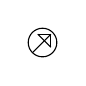
\begin{tikzpicture}
        \draw (0,0) circle (1.2ex);
        \draw (0.7 ex, 0.7 ex) -- (-0.4 ex, 0.7 ex);
        \draw (-0.4 ex, 0.7 ex) -- (0.7 ex, -0.4 ex);
        \draw (0.7 ex, -0.4 ex) -- (0.7 ex, 0.7 ex);
        \draw (0.7 ex, 0.7 ex) -- (-0.848 ex, -0.848 ex);
    \end{tikzpicture}}}
    \ \ 
}

% legendre符号
\makeatletter
\def\legendre@dash#1#2{\hb@xt@#1{%
  \kern-#2\p@
  \cleaders\hbox{\kern.5\p@
    \vrule\@height.2\p@\@depth.2\p@\@width\p@
    \kern.5\p@}\hfil
  \kern-#2\p@
  }}
\def\@legendre#1#2#3#4#5{\mathopen{}\left(
  \sbox\z@{$\genfrac{}{}{0pt}{#1}{#3#4}{#3#5}$}%
  \dimen@=\wd\z@
  \kern-\p@\vcenter{\box0}\kern-\dimen@\vcenter{\legendre@dash\dimen@{#2}}\kern-\p@
  \right)\mathclose{}}
\newcommand\legendre[2]{\mathchoice
  {\@legendre{0}{1}{}{#1}{#2}}
  {\@legendre{1}{.5}{\vphantom{1}}{#1}{#2}}
  {\@legendre{2}{0}{\vphantom{1}}{#1}{#2}}
  {\@legendre{3}{0}{\vphantom{1}}{#1}{#2}}
}
\def\dlegendre{\@legendre{0}{1}{}}
\def\tlegendre{\@legendre{1}{0.5}{\vphantom{1}}}
\makeatother
\addbibresource{Accessories/ref.bib}
\newcommand{\Yang}[1]{\textcolor{red}{#1}}


\title{Notes in Algebraic Geometry}
\author{Tianle Yang}
\date{\today}
\authoremail{\href{mailto:loveandjustice@88.com}{loveandjustice@88.com}}
\authorpage{\href{https://www.tianleyang.com}{tianleyang.com}}
\texsource{\href{https://github.com/MonkeyUnderMountain/Note_on_Algebraic_Geometry}{github.com/MonkeyUnderMountain/Note\_on\_Algebraic\_Geometry}}
\version{0.1.0}

\setCJKfamilyfont{lxgwwenkai}{LXGW WenKai} % 定义霞鹜文楷,若未安装,请去掉相关代码编译或使用其他字体
\coversentence{\CJKfamily{lxgwwenkai}「あんたバかァ?」}
\coverimage{Asuka.png} % 封面图片
\coverlinecolor{brown!80!yellow} % 封面横线颜色
\covertitlefont{Allura} % 封面标题字体, 若未安装,可注释掉此行编译或使用其他字体
\covertextcolor{red!80!black} % 封面标题颜色


\begin{document}

    % \pagestyle{empty}
    \maketitle

    \frontmatter

    \tableofcontents

    \mainmatter

    % \chapter{The First Properties}
    %     \section{Setup and the first examples}

    Let $S$ be a locally noetherian and separated scheme.
    An $S$-variety is a separated scheme $X$ which is of finite type and flat over $S$.

    We will use $\mathsf{k},\mathsf{K}$ to denote fields, and $\mathbf{k},\mathbf{K}$ to denote their algebraically closure relatively.
    Let $X$ be an integral scheme.
    We denote by $\KK(X)$ the function field of $X$.
    For a closed point $x \in X$, we denote by $\mathsf{k}(x)$ the residue field of $x$.
    We denote the category of $S$-varieties by $\Var_S$.
    We denote by $X(T)$ the set of $T$-points of $X$, that is, the set of morphisms $T \to X$.


\begin{example}
    Let $\kkk$ be an algebraically closed field and $A$ the localization of $\kkk[x]$ at $(x)$.
    Let $S = \Spec A$ and $X = \Spec A[y]$. 
    There are three types of points in $X$:
    \begin{enumerate}[label=(\roman*)]
        \item closed points with residue field $\kkk$, like $p = (x,y-a)$;
        \item closed points with residue field $\kkk(y)$, like $P = (xy-1)$;
        \item non-closed points, like $\eta_1 = (x),\eta_2 = (y),\eta_3 = (x-y)$.
    \end{enumerate}

\end{example}
 
    %     % \section{Normality and Cohen-Macaulay schemes}

\subsection{Height, Depth and Dimension}

    \paragraph{Krull dimension and height of prime ideals}

    Algebraically, we have following definitions.
    \begin{definition}
        Let $A$ be a noetherian ring.
        The \textit{height of a prime ideal} $\frakp$ in $A$ is defined as the maximum length of chains of prime ideals contained in $\frakp$, that is, 
        \[ \idealht(\frakp) := \sup\{ n \mid \exists \text{ a chain of prime ideals } \frakp_0 \subsetneq \frakp_1 \subsetneq \cdots \subsetneq \frakp_n = \frakp\}. \] 
        The \textit{Krull dimension} of $A$ is defined as 
        \[ \dim A := \max_{\frakp \in \Spec A}\idealht(\frakp). \]
    \end{definition}

    Geometrically, we have the corresponding definition.
    \begin{definition}
        Let $X$ be a noetherian scheme.
        The \textit{codimension of a irreducible subscheme} $Y$ in $X$ is defined as the length of the longest chain of irreducible closed subsets containing $Y$, that is, 
        \[ \codim_X(Y) := \sup\{ n \mid \exists \text{ a chain of irreducible closed subsets } Y = Y_0 \subsetneq Y_1 \subsetneq \cdots \subsetneq Y_n\}. \] 
        The \textit{dimension} of $X$ is defined as
        \[ \dim X := \max_{Y \in \text{Irred}(X)}\codim_X(Y). \]
    \end{definition}

    For an affine schemes $X = \Spec A$, above two definitions coincide by the correspondence of prime ideals and irreducible closed subsets.

    \begin{proposition}
        Let $A$ be a noetherian ring and $\frakp \in \Spec A$.
        Then the height of $\frakp$ is equal to the codimension of the irreducible closed subset $V(\frakp)$ in $\Spec A$.
    \end{proposition}

    For "nice" schemes, the Krull dimension behaves well by following proposition.

    \begin{proposition}
        Let $S$ be spectrum of a field $\kk$ or an algebraic integer ring $\calo_K$ and $X$ an integral $S$-variety.
        Then we have the follows:
        \begin{enumerate}[label=(\roman*)]
            \item For any point $P \in X$, $\dim X = \dim \calo_{X,P} + \codim \overline{\{P\}}$.
            \item For any non-empty open subset $U \subset X$, $\dim U = \dim X$.
            \item $\dim X = \operatorname{trdeg}(\fkk(X)/\fkk(S)) + \dim S$.
        \end{enumerate}
    \end{proposition}


    \paragraph{Depth}

    For a noetherian local ring $(A,\frakm)$, we can define the depth of an $A$-module $M$.

    \begin{definition}
        Let $(A,\frakm)$ be a noetherian local ring with residue field $\kk$ and $M$ a finitely generated $A$-module. 
        A sequence $t_1,\cdots,t_n\in \frakm$ is called a \textit{regular sequence for $M$} if $t_i$ is not a zero divisor on $M/(t_1,\cdots,t_{i-1})$, that is, $M/(t_1,\cdots,t_{i-1}) \to t_iM/(t_1,\cdots,t_{i-1})$ is injective.
        The \textit{depth} of $M$ is defined as the maximum length of regular sequences for $M$.
    \end{definition}

    Up to now, there are three numbers measuring the ``size'' of a local ring $(A,\frakm)$:
    \begin{itemize}
        \item $\dim A$: the Krull dimension of $A$.
        \item $\depth A$: the depth of $A$.
        \item $\dim_{\rkk(\frakm)} T_{A,\frakm}$: the dimension of Zariski tangent space $T_{A,\frakm} := (\frakm/\frakm^2)^\lor$ as a ${\rkk(\frakm)}$-vector space.
    \end{itemize}

    These three numbers are related by the following inequalities.
    \begin{proposition}
        Let $(A,\frakm)$ be a local noetherian ring with residue field $\kk$.
        Then the following inequalities hold:
        \[ \depth A \leq \dim A \leq \dim_\kk T_{A,\frakm}. \]
    \end{proposition}

    To see these, we need the following well-known theorem.

    
    \begin{theorem}[Krull's Principal Ideal Theorem]
        % Let $(A,\frakm)$ be a local noetherian ring with residue field $\kk$.
        % Then the following inequalities hold:
        % \[ \dim A \leq \dim_\kk T_{A,\frakm} \leq \dim A + \dim_\kk \kappa(\frakm) - 1. \]
    \end{theorem}

    \begin{theorem}[Nakayama's Lemma]
        thhhhh
    \end{theorem}

\subsection{Normal schemes}

    % Fix a noetherian local ring $(A,\frakm)$ with residue field $\kk$.

    \begin{definition}
        A ring $A$ is called \textit{normal} if it is an integral domain and integrally closed in its field of fractions $\Frac(A)$.
    \end{definition}

    \begin{proposition}
        Normality is a local property. 
        That is, TFAE:
        \begin{enumerate}[label=(\alph*)]
            \item $A$ is normal.
            \item For any prime ideal $\frakp \in \Spec A$, the localization $A_\frakp$ is normal.
            \item For any maximal ideal $\frakm \in \mSpec A$, the localization $A_\frakm$ is normal.
        \end{enumerate}
    \end{proposition}
    \begin{proof}
        
    \end{proof}

    \begin{proposition}
        Let $A$ be a normal ring.
        Then $A[X]$ and $A[[X]]$ are normal rings.
    \end{proposition}

    \begin{definition}
        A scheme $X$ is called \textit{normal} if the local ring $\calo_{X,x}$ is normal for any point $x\in X$.
    \end{definition}

    \begin{example}
        
    \end{example}

    \begin{definition}
        Let $X$ be a scheme.
        The \textit{normalization} of $X$ is a $X$-scheme $X^\nu$ with the following universal property:
        for any normal $X$-scheme $Y$, its structure morphism $Y \to X$ factors through $X^\nu$.
    \end{definition}

    \begin{proposition}
        Let $X$ be an integral scheme.
        Then the normalization $X^\nu$ of $X$ exists.
        Moreover, $X^\nu \to X$ is birational.
    \end{proposition}

    \begin{theorem}
        Let $X$ be a normal noetherian scheme.
        Let $F \subset X$ be a closed subset of codimension $\geq 2$.
        Then the restriction $H^0(X,\calo_X) \to H^0(X\setminus F, \calo_{X})$ is an isomorphism.
    \end{theorem}


    
\subsection{Regular conditions and Serre's conditions}

    \begin{definition}
        Let $X$ be a locally noetherian scheme and $k \in \bbz_{\geq 0}$.
        We say that \textit{$X$ verifies property $R_k$} or \textit{is regular in codimension $k$} if $\forall \xi \in X$ with $\codim \overline{\{\xi\}} \leq k$, 
        \[ \dim_{\rkk(\xi)} T_{X,\xi} = \dim \calo_{X,\xi}. \]
        We say that \textit{$X$ verifies property $S_k$} if $\forall \xi \in X$,
        \[ \depth \calo_{X,\xi} \geq \min\{k, \dim \calo_{X,\xi}\}. \]        
    \end{definition}

    \begin{definition}[Cohen-Macaulay]
        A noetherian local ring $(A,\frakm)$ is called \textit{Cohen-Macaulay} if $\dim A = \depth A$.
        A locally noetherian scheme $X$ is called \textit{Cohen-Macaulay} if $\calo_{X,\xi}$ is Cohen-Macaulay for any point $\xi \in X$.
    \end{definition}

    By definition, it is easy to see that $X$ is Cohen-Macaulay if and only if it verifies $S_k$ for all $k \geq 0$.

    \begin{example}[Non Cohen-Macaulay rings]

    \end{example}

    \begin{definition}
        % We say that the unmixedness theorem holds for a noetherian ring $A$ if 
        An ideal $I$ of a noetherian ring $A$ is called \textit{unmixed} if 
        \[ \idealht(I) = \idealht(\frakp), \quad \forall \frakp \in \Ass(A/I). \]
        We say that \textit{the unmixedness theorem holds for a noetherian ring $A$} if any ideal $I \subset A$ generated by $\idealht(I)$ elements is unmixed.
        We say that \textit{the unmixedness theorem holds for a locally noetherian scheme $X$} if $\calo_{X,\xi}$ is unmixed for any point $\xi \in X$.
    \end{definition}

    \begin{remark}
        Recall that the set of associated primes of a module $M$ is defined as
        \[ \Ass(M) := \{ \frakp \in \Spec A \colon \exists x \in M \text{ such that } \frakp = \Ann(x) \}. \] 
        
    \end{remark}

    \begin{theorem}
        Let $X$ be a locally noetherian scheme.
        Then the unmixedness theorem holds for $X$ if and only if $X$ is Cohen-Macaulay.
    \end{theorem}

    \begin{proposition}
        
    \end{proposition}


    \begin{theorem}[Serre's criterion for normality]
        Let $X$ be a 
    \end{theorem}
    

    \chapter{Schemes and Varieties}
        \section{Definition and First Properties}


\subsection{Locally Ringed Space}


\subsection{Schemes}

    \begin{example}[Glue open subschemes]\label{eg:glue_open_subschemes}
        We construct a scheme by gluing open subschemes.
        Let \(X_i\) be schemes for \(i \in I\) and \(U_{ij} \subseteq X_i\) be open subschemes for \(i,j \in I\).
        Suppose we have isomorphisms \(\varphi_{ij} : U_{ij} \to U_{ji}\) such that
        \begin{enumerate}
            \item \(\varphi_{ii} = \id_{X_i}\) for all \(i \in I\);
            \item \(\varphi_{ij}(U_{ij} \cap U_{ik}) = U_{ji} \cap U_{jk}\) for all \(i,j \in I\);
            \item \(\varphi_{jk}\circ \varphi_{ij} = \varphi_{ik}\) on \(U_{ij} \cap U_{ik}\) for all \(i,j,k \in I\).
        \end{enumerate}
        \Yang{}
    \end{example}

        \section{Linear Systems}


\subsection{Sections, linear systems and morphisms to projective space}

    \begin{theorem}\label{thm:morphism_to_projective_space}
        Let \(A\) be a ring and \(X\) an \(A\)-scheme.
        Let \(\calL\) be a line bundle on \(X\) and \(s_0,\ldots,s_n\in\Gamma(X,\calL)\).
        Suppose that \(\{s_i\}\) generate \(\calL\), i.e., \(\bigoplus_i \calO_X s_i \to \calL\) is surjective.
        Then there is a unique morphism \(f:X\to \bbP^n_A\) such that \(\calL\cong f^*\calO(1)\) and \(s_i=f^*x_i\), where \(x_i\) are the standard coordinates on \(\bbP^n_A\).   
    \end{theorem}
    \begin{proof}
        \Yang{To be continued.}
    \end{proof}


\subsection{Asymptotic behavior of linear systems}


\subsection{Iitaka fibration}

    \chapter{Surfaces}
        \section{Ruled Surface}

In this section, fix an algebraically closed field $\kkk$.

\subsection{Preliminaries}

    Let \(S\) be a variety over \(\kkk\) and \(\calE\) a vector bundle of rank \(r+1\) on \(S\).

    \begin{proposition}\label{prop:isomorphic_projective_bundle_iff_twist_by_line_bundle}
        The \(S\)-varieties \(\bbP_X(\calE) \cong \bbP_X(\calE')\) if and only if \(\calE \cong \calE' \otimes \calL\) for some line bundle \(\calL\) on \(S\).
    \end{proposition}

    \begin{theorem}\label{thm:Eulur_sequence_for_projective_bundle}
        Let \(\pi: X=\bbP_S(\calE) \to S\) be the projective bundle associated to a vector bundle \(\calE\) of rank \(r+1\) on \(S\). 
        Then there is an exact sequence of vector bundles on \(\bbP_S(\calE)\)
        \[
            0 \to \Omega_{\bbP_S(\calE)/S} \to \pi^*(\calE)(-1) \to \calO_{\bbP_S(\calE)} \to 0.
        \]
        In particular, \(K_X \sim \pi^*(K_S + \det \calE) - (r+1)\calO_{\bbP_S(\calE)}(1)\).
        \Yang{To be continued...}
    \end{theorem}

    \begin{theorem}[Tsen's Theorem, {\cite[Tag 03RD]{Stacks}}]\label{thm:Tsen_theorem}
        Let \(C\) be a smooth curve over an algebraically closed field \(\kkk\). 
        Then \(\KK=\kkk(C)\) is a \(C_1\) field, i.e., every degree \(d\) hypersurface in \(\bbP^n_{\KK}\) has a \(\KK\)-rational point provided \(d \leq n\).
        % \Yang{Need a reference.}
    \end{theorem}

    % \begin{theorem}[Cohomology and Base Change, {\cite[Theorem 12.11]{Har77}}]\label{thm:cohomology_and_base_change}
    %     Let \(f:X \to S\) be a projective morphism of noetherian schemes and \(\calF\) a coherent sheaf on \(X\) which is flat over \(S\). 
    %     Then for each \(i \geq 0\) and each point \(s \in S\) there is a natural base change homomorphism
    %     \[
    %         \varphi_s^i: \sfR^i f_*\calF \ten_{\calO_S} \rkk(s) \to H^i(X_s,\calF_s).
    %     \]
    %     Suppose that \(\varphi_s^i\) is surjective. 
    %     Then
    %     \begin{enumerate}
    %         \item there exists an open neighborhood \(U\) of \(s\) such that \(\varphi_{s'}^i\) is an isomorphism for all \(s' \in U\);
    %         \item TFAE:
    %             \begin{enumerate}
    %                 \item \(\varphi_{s}^{i-1}\) is surjective;
    %                 \item \(\sfR^i f_*\calF\) is locally free on an open neighborhood of \(s\).
    %             \end{enumerate}
    %     \end{enumerate}
    % \end{theorem}

    \begin{theorem}[Grauert's Theorem, {\cite[Corollary 12.9]{Har77}}]\label{thm:Grauert_theorem}
        Let \(f:X \to S\) be a projective morphism of noetherian schemes and \(\calF\) a coherent sheaf on \(X\) which is flat over \(S\).
        Suppose that \(S\) is integral and the function \(s \mapsto \dim_{\rkk(s)} H^i(X_s,\calF_s)\) is constant on \(S\) for some \(i \geq 0\). 
        Then \(\sfR^i f_*\calF\) is locally free and the base change homomorphism
        \[
            \varphi_s^i: \sfR^i f_*\calF \ten_{\calO_S} \rkk(s) \to H^i(X_s,\calF_s)
        \]
        is an isomorphism for all \(s \in S\).
    \end{theorem}

    \begin{theorem}[Miracle Flatness, {\cite[Theorem 23.1]{Mat89}}]\label{thm:miracle_flatness}
        Let \(f:X \to Y\) be a morphism of noetherian schemes. 
        Assume that \(Y\) is regular and \(X\) is Cohen-Macaulay. 
        If all fibers of \(f\) have the same dimension \(d = \dim X - \dim Y\), then \(f\) is flat.
    \end{theorem}

    \begin{proposition}[Geometric form of Nakayama's Lemma]\label{prop: geometric form of Nakayama's lemma}
        Let \(X\) be a variety, $x\in X$ a closed point and $\calF$ a coherent sheaf on $X$.
        If $a_1,\cdots,a_k \in \calF(X)$ generate $\calF|_x = \calF \ten \rkk(x)$, then there is an open subset $U \subset X$ such that $a_i|_U$ generate $\calF(U)$. 
    \end{proposition}

    \begin{proposition}\label{prop:relative_projective_morphism}
        Let \(S\) be a noetherian scheme and \(\calE\) a vector bundle of rank \(r+1\) on \(S\). 
        % Then the projection \(\pi:\bbP_X(\calE) \to X\) is a projective morphism.
        Let \(X\) be a \(S\)-scheme via a morphism \(g:X \to S\).
        Then there is a bijection
        \[
            \{S\text{-morphisms } X \to \bbP_S(\calE)\}
            \leftrightarrow
            \left\{
                \begin{array}{l}
                    \text{surjective homomorphisms } g^*\calE \to \calL \\
                    \text{where } \calL \text{ is a line bundle on } X
                \end{array}
            \right\}.
        \]
        \Yang{Need to check.}
    \end{proposition}
    \begin{proof}
        Take an affine cover \(\{U_i\}\) of \(S\) such that \(\calE|_{U_i}\) is trivial.
        On \(U_i\), the surjection \(g^*\calE|_{U_i} \surjmap \calL|_{X_{U_i}}\) gives a morphism \(X_{U_i} \to \bbP_{U_i}(\calE|_{U_i}) \cong \bbP_{S}(\calE)_{U_i}\) by \Yang{ref}.

    \end{proof}

\subsection{Minimal Section and Classification}

    \begin{definition}[Ruled surface]\label{def:ruled_surface}
        A \emph{ruled surface} is a smooth projective surface \(X\) together with a surjective morphism \(\pi:X \to C\) to a smooth curve \(C\) such that all fibers of \(\pi\) are isomorphic to \(\bbP^1\).
    \end{definition}

    Let \(\pi:X \to C\) be a ruled surface over a smooth curve \(C\) of genus \(g\).


    \begin{lemma}\label{lem:existence_of_section_of_ruled_surface}
        There exists a section of \(\pi\).
    \end{lemma}
    \begin{proof}
        \Yang{To be continued...}
    \end{proof}

    \begin{proposition}\label{prop:ruled_surface_as_projective_bundle}
        % Let \(\pi:X \to C\) be a ruled surface over a smooth curve \(C\). 
        Then there exists a vector bundle \(\calE\) of rank \(2\) on \(C\) such that \(X \cong \bbP_C(\calE)\) over \(C\).
    \end{proposition}
    \begin{proof}
        Let \(\sigma:C \to X\) be a section of \(\pi\) and \(D\) be its image.
        Let \(\calL = \calO_X(D)\) and \(\calE = \pi_*\calL\).
        Since \(D\) is a section of \(\pi\), \(\calL|_{X_t} \cong \calO_{\bbP^1}(1)\) for any \(t \in C\), whence \(h^0(X_t,\calL|_{X_t}) = 2\) for any \(t \in C\).
        By Miracle Flatness (\cref{thm:miracle_flatness}), \(f\) is flat.
        By Grauert's Theorem (\cref{thm:Grauert_theorem}), \(\calE\) is a vector bundle of rank \(2\) on \(C\) and we have a natural isomorphism \(\calE \ten \rkk(t) \cong H^0(X_t,\calL|_{X_t})\) for any \(t \in C\).

        This gives a surjective homomorphism 
        \[ \calE \ten_{\calO_C} \rkk(t) \ten_{\rkk(t)} \calO_{X_t} \cong H^0(X_t,\calL|_{X_t}) \ten_{\rkk(t)} \calO_{X_t} \surjmap \calL|_{X_t}. \]
        For every \(x \in X\), we have 
        \[ \calE \ten_{\calO_C} \rkk(\pi(x)) \ten_{\rkk(\pi(x))} \calO_{X_{\pi(x)}} \ten_{\calO_{X_{\pi(x)}}} \rkk(x)  \surjmap \calL|_{X_{\pi(x)}}\ten_{\calO_{X_{\pi(x)}}} \rkk(x). \]
        \Yang{The left side coincides with \(\pi^*\calE\ten_{\calO_X} \rkk(x)\) naturally.}
        Hence by Nakayama's Lemma, the natural homomorphism \(\pi^*\calE \to \calL\) is surjective.

        Denote by \(p: \bbP_C(\calE) \to C\) the projection.
        Take an affine open cover \(\{U_i\}\) of \(C\) such that \(\calE|_{U_i}\) is trivial.
        On \(U_i\), the surjection \(\pi^*\calE|_{X_{U_i}} \surjmap \calL|_{X_{U_i}}\) gives a morphism \(\varphi_i: X_{U_i} \to \bbP_{U_i}(\calE|_{U_i}) \cong \bbP_{C}(\calE)_{U_i}\) by \Yang{ref}.
        Since \(\varphi_i\) and \(\varphi_j\) agree on \(X_{U_i \cap U_j}\), they glue to give a morphism \(\varphi:X \to \bbP_C(\calE)\) over \(C\).
        Since \(\varphi|_{X_t}:X_t \to \bbP_C(\calE)_t\) is an isomorphism for any \(t \in C\), \(\varphi\) is 
        % Since both \(X\) and \(\bbP_C(\calE)\) are smooth, \(\varphi\) is an isomorphism.
    \end{proof}

    \begin{lemma}\label{lem:correspondence_between_sections_and_quotient_line_bundles}
        Fix a vector bundle \(\calE\) of rank \(2\) on \(C\) such that \(X \cong \bbP_C(\calE)\).
        There is a one-to-one correspondence between sections of \(\pi\) and quotient line bundles of \(\calE\) on \(\calC\).
    \end{lemma}
    \begin{proof}
        Suppose we have a quotient \(\calE \to \calL \to 0\) on \(C\) where \(\calL\) is a line bundle on \(C\).
        By \cref{prop:relative_projective_morphism}, we have a morphism \(s:C \to \bbP_C(\calE)\) over \(C\).
        Conversely, let \(\sigma:C \to X\) be a section of \(\pi\) and \(D\) be its image.
    \end{proof}

    \begin{lemma}\label{lem:existence_of_normalized_vector_bundle}
        It is possible to write \(X \cong \bbP_C(\calE)\) such that \(H^0(C,\calE) \neq 0\) but \(H^0(C,\calE \otimes \calL) = 0\) for any line bundle \(\calL\) on \(C\) with \(\deg \calL < 0\).
        Such a vector bundle \(\calE\) is called a \emph{normalized vector bundle}.
    \end{lemma}
    \begin{proof}
        
    \end{proof}

    \begin{definition}\label{def:minimal_section_of_ruled_surface}
        A section \(C_0\) of \(\pi\) is called a \emph{minimal section} if \Yang{to be continued...}
    \end{definition}

    \begin{lemma}\label{thm:restriction_of_e}
        Let \(X=\bbP_C(\calE) \to C\) be a ruled surface over a smooth curve \(C\) of genus \(g\) with invariant \(e\) and normalized \(\calE\). 
        \begin{enumerate}
            \item If \(\calE\) is decomposable, then \(e \geq 0\) and \(\calE \cong \calO_C \oplus \calL\) where \(\calL\) is a line bundle on \(C\) with \(\deg \calL = -e\).
            \item If \(\calE\) is indecomposable, then \(-2g \leq e \leq 2g - 2\).
        \end{enumerate} 
    \end{lemma}

    \begin{theorem}\label{thm:classification_of_ruled_surface_on_P1}
        Let \(\pi:X \to C\) be a ruled surface over \(C = \bbP^1\) with invariant \(e\).
        Then \(X \cong \bbP_{C}(\calO_C \oplus \calO_C(-e))\).
    \end{theorem}

    \begin{example}\label{eg:explicit_description_of_rational_ruled_surface}
        Here we give an explicit description of the ruled surface \(X = \bbP_{\bbP^1}(\calO \oplus \calO(-e))\) for \(e \geq 0\).
        \Yang{To be continued...}
    \end{example}

    \begin{theorem}\label{thm:classification_of_ruled_surface_on_elliptic_curve}
        Let \(\pi:X = \bbP_E(\calE) \to E\) be a ruled surface over an elliptic curve \(E\) with invariant \(e\) and normalized \(\calE\). 
        \begin{enumerate}
            \item If \(\calE\) is indecomposable, then \(e = 0\) or \(-1\), and for each \(e\) there exists a unique such ruled surface up to isomorphism.
            \item If \(\calE\) is decomposable, then \(e \geq 0\) and \(\calE \cong \calO_E \oplus \calL\) where \(\calL\) is a line bundle on \(E\) with \(\deg \calL = -e\).
        \end{enumerate}
    \end{theorem}

    \begin{example}
        \Yang{To be continued...}
    \end{example}


\subsection{The N\'eron-Severi Group of Ruled Surfaces}

    \begin{proposition}\label{prop:Picard_group_of_ruled_surface}
        Let \(\pi:X \to C\) be a ruled surface over a smooth curve \(C\) of genus \(g\). 
        Let \(C_0\) be a minimal section of \(\pi\) and let \(f\) be a fiber of \(\pi\). 
        Then \(\Pic(X) \cong \bbZ C_0 \oplus \pi^*\Pic(C)\).
        \Yang{Check this carefully.}
    \end{proposition}
    \begin{proof}
        \Yang{To be continued...}
    \end{proof}

    \begin{proposition}\label{prop:canonical_divisor_of_ruled_surface}
        Let \(\pi:X \to C\) be a ruled surface over a smooth curve \(C\) of genus \(g\). 
        Let \(C_0\) be a minimal section of \(\pi\) and let \(f\) be a fiber of \(\pi\). 
        Then \(K_X \sim -2C_0 + (K_C-)f\) where \(e = -C_0^2\).
        \Yang{Check this carefully.}
    \end{proposition}
    \begin{proof}
        \Yang{To be continued.}
    \end{proof}

    \paragraph{Rational case.} Let \(\pi:X = \bbP_{\bbP^1}(\calE) \to \bbP^1\) be a ruled surface over \(\bbP^1\) with \(\calE \cong \calO \oplus \calO(-e)\) for some \(e \geq 0\).

    \begin{theorem}\label{thm:positivity_of_divisors_on_rational_ruled_surface}
        Let \(\pi:X \to \bbP^1\) be a ruled surface over \(\bbP^1\) with invariant \(e\).
        Let \(C_0\) be a minimal section of \(\pi\) and let \(F\) be a fiber of \(\pi\). 
        Let \(D \sim aC_0 + bF\) be a divisor on \(X\) with \(a,b \in \bbZ\).
        \begin{enumerate}
            \item \(D\) is ample \(\iff\) \(D\) is very ample \(\iff\) \(a > 0\) and \(b > ae\);
            \item \(D\) is effective \(\iff\) \(a,b \geq 0\).
        \end{enumerate} 
    \end{theorem}
    \begin{proof}
        \Yang{To be continued...}
    \end{proof}


    \paragraph{Elliptic case.} Let \(\pi:X = \bbP_C(\calE) \to E\) be a ruled surface over an elliptic curve \(E\) with \(\calE\) a normalized vector bundle of rank \(2\) and degree \(-e\).

    \begin{theorem}\label{thm:positivity_of_divisors_on_decomposable_ruled_surface_over_elliptic_curve}
        Let \(\pi:X \to E\) be a ruled surface over an elliptic curve \(E\) with invariant \(e\).
        Assume that \(\calE\) is decomposable.
        Let \(C_0\) be a minimal section of \(\pi\) and let \(F\) be a fiber of \(\pi\). 
        Let \(D \equiv aC_0 + bF\) be a divisor on \(X\) with \(a,b \in \bbZ\).
        \begin{enumerate}
            \item \(D\) is ample \(\iff\) \(D\) is very ample \(\iff\) \(a > 0\) and \(b > ae\);
            \item \(D\) is effective \(\iff\) \(a \geq 0\) and \(b \geq ae\).
        \end{enumerate}
    \end{theorem}
    \begin{proof}
        \Yang{To be continued...}
    \end{proof}

    \begin{theorem}\label{thm:positivity_of_divisors_on_indecomposable_ruled_surface_over_elliptic_curve}
        Let \(\pi:X \to E\) be a ruled surface over an elliptic curve \(E\) with invariant \(e\).
        Assume that \(\calE\) is indecomposable.
        Let \(C_0\) be a minimal section of \(\pi\) and let \(F\) be a fiber of \(\pi\). 
        Let \(D \equiv aC_0 + bF\) be a divisor on \(X\) with \(a,b \in \bbZ\).
        \begin{enumerate}
            \item \(D\) is ample \(\iff\) \(D\) is very ample \(\iff\) \(a > 0\) and \(b > \frac{1}{2}ae\);
            \item \(D\) is effective \(\iff\) \(a \geq 0\) and \(b \geq \frac{1}{2}ae\).
        \end{enumerate}
    \end{theorem}
    \begin{proof}
        \Yang{To be continued...}
    \end{proof}



    \chapter{Birational Geometry}
        \section{here is the text}

    \lipsum[3-4]

\subsection{theorems and definitions}
    \lipsum[5-6]

   

    \begin{definition}[this is a definition]
        \lipsum[1-2]    
    \end{definition}
    \begin{proposition}[this is a proposition]
        \lipsum[1-2] 
    \end{proposition}
    \begin{example}[this is an example]
        \lipsum[1-2] 
    \end{example}
    \begin{theorem}[this is a theorem]
        \lipsum[1-2] 
    \end{theorem}
    \begin{corollary}[this is a corollary]
        \lipsum[1-2] 
    \end{corollary}
    \begin{exercise}[this is an exercise]
        \lipsum[1-2]
    \end{exercise}
    \begin{remark}[this is a remark]
        \lipsum[1-2]
    \end{remark}
    \begin{proof}[this is a proof]
        \lipsum[1-2]
    \end{proof}
    \begin{lemma}[this is a lemma]
        \lipsum[1-2]
    \end{lemma}

    \lipsum[100-200] % 生成测试文本

        \section{Kodaira Vanishing Theorem}

\subsection{Preliminary}

    % \begin{theorem}[GAGA]\label{thm: GAGA for cohomology}
    %     Let $X$ be a smooth projective variety over $\mathbb{C}$ and \(\calf\) a coherent sheaf on \(X\).
    %     Then 
    %     \[
    %         H^i(X, \calf) \cong H^i(X^{an}, \calf^{an}).
    %     \]
    % \end{theorem}

    \begin{theorem}[Serre Duality]\label{thm: Serre duality for line bundles}
        Let \(X\) be a Cohen-Macaulay projective variety of dimension \(n\) over \(\kk\) and \(D\) a divisor on \(X\).
        Then there is an isomorphism
        \[
            H^i(X, D) \cong H^{n-i}(X, K_X - D)^\vee, \quad \forall i = 0, 1, \ldots, n.
        \]
    \end{theorem}

    % \begin{theorem}[Serre Vanishing]\label{thm: Serre vanishing theorem}
    %     Let \(X\) be a proper variety of dimension \(n\) over \(\kk\), \(\calf\) a coherent sheaf and \(\call\) an ample line bundle on \(X\). 
    %     Then there exists an integer \(m_0 > 0\) such that for all \(m \geq m_0\),
    %     \[
    %         H^i(X, L^m\ten \calf) = 0,\quad \forall i > 0.
    %     \]
    % \end{theorem}

    \begin{theorem}[Log Resolution of Singularities]\label{thm: log resolution of singularities}
        Let X be an irreducible reduced algebraic variety over $\bbc$ (or a suitably small neighborhood of a compact set of an irreducible reduced analytic space) and $I \subset \calo_X$ a coherent sheaf of ideals defining a closed subscheme (or subspace) $Z$. Then there is a smooth variety (or analytic space) $Y$ and a projective morphism $f: Y \to X$ such that
        \begin{enumerate}
            \item $f$ is an isomorphism over $X - (\Sing(X) \cup \Supp Z)$,
            \item $f^*I \subset \calo_Y$ is an invertible sheaf $\calo_Y(-D)$ and 
            \item $\Exc(f) \cup D$ is an snc divisor.
        \end{enumerate}
    \end{theorem}

    \begin{theorem}[Lefschetz Hyperplane Theorem]\label{thm: Lefschetz hyperplane theorem}
        Let \(X\) be a smooth projective variety of dimension \(n\) over \(\bbc\) and \(Y\) a hyperplane section of \(X\).
        Then the restriction map
        \[
            H^k(X,\bbc) \to H^k(Y, \bbc)
        \]
        is an isomorphism for \(k < n - 1\) and an injection for \(k = n - 1\).
    \end{theorem}

    \begin{theorem}[Hodge Decomposition]\label{thm: Hodge decomposition}
        Let \(X\) be a smooth projective variety of dimension \(n\) over \(\bbc\).
        Then for any \(k\), there is a functorial decomposition
        \[
            H^k(X, \bbc) = \bigoplus_{p+q=k} H^{p}(X, \Omega^q_X).
        \]
    \end{theorem}

    Combine Theorem \ref{thm: Lefschetz hyperplane theorem} and Theorem \ref{thm: Hodge decomposition}, we have the following lemma.

    \begin{lemma}\label{lem: Lefschetz hyperplane theorem for cohomology of structure sheaf}
        Let \(X\) be a smooth projective variety of dimension \(n\) over \(\bbc\) and \(Y\) a hyperplane section of \(X\).
        Then the restriction map \(r_k: H^k(X,\bbc) \to H^k(Y, \bbc)\) decomposes as 
        \[
            r_k = \bigoplus_{p+q=k} r_{p,q},\quad r_{p,q}: H^{p}(X, \Omega^q_X) \to H^{p}(Y, \Omega^q_Y).
        \]
        And \(r_{p,q}\) is an isomorphism for \(p + q < n - 1\) and an injection for \(p + q = n - 1\).
        In particular, 
        \[ H^p(X, \calo_X) \to H^p(Y, \calo_Y) \]
        is an isomorphism for \(p < n - 1\) and an injection for \(p = n - 1\).
    \end{lemma}

    \begin{theorem}[Leray spectral sequence]\label{thm: Leray spectral sequence}
        Let \(f: Y \to X\) be a morphism of varieties and \(\calf\) a coherent sheaf on \(Y\).
        Then there is a spectral sequence
        \[
            E_2^{p,q} = H^p(X, R^q f_* \calf) \implies H^{p+q}(Y, \calf).
        \]
    \end{theorem}
        

\subsection{Kodaira Vanishing Theorem}

    \begin{lemma}\label{lem: cyclic covering map in Kodaira Vanishing}
        Let \(X\) be a smooth projective variety over \(\kk\) and \(\call\) a line bundle on \(X\).
        Suppose there is an integer \(m\) and a smooth divisor \(D \in H^0(X, \call^m)\).
        Then there exists a finite surjective morphism \(f:Y \to X\) of smooth projective varieties such that \(D':= f^{-1}(D)\) is smooth and satisfies that \(bD' = af^*D\).
    \end{lemma}
    \begin{proof}
        Let \(s \in \call^m\) be the section defining \(D\).
        It induces a homomorphism \(\call^{-m} \to \calo_X\).
        Consider the \(\calo_X\)-algebra 
        \[ \cala := \left(\bigoplus_{i = 0}^{\infty} \call^{-i}\right) \bigg/\left(\call^{-m} \to \calo_X\right) \cong \bigoplus_{i = 0}^{m-1} \call^{-i}. \]
        Then \(\cala\) is a finite \(\calo_X\)-algebra.
        Let \(Y \coloneqq \Spec_X \cala\).
        Then \(Y\) is a finite \(\calo_X\)-scheme and the natural morphism \(f: Y \to X\) is finite and surjective.

        For every \(x \in X\), let \(\call\) locally generated by \(t\) near \(x\).
        Then \(\calo_Y\) locally equal to \(\calo_X[t]/(t^m - s)\).
        Let \(D'\) be the divisor locally given by \(t=0\) on \(Y\).
        Since \(X\) and \(D\) are smooth, then \(Y\) is a smooth variety and \(D'\) is smooth.
        Since \(f\) is finite, it is proper.
        Then \(Y\) is proper and hence \(Y\) is projective.
    \end{proof}
    \begin{remark}\label{rmk: cyclic covering map in Kodaira Vanishing can preverse snc}
        Let \(D_i\) be reduced effective divisors on \(X\) such that \(D + \sum_{i=1}^k D_i\) is snc.
        Set \(D_i' = f^*(D_i)\).
        Then \(D' + \sum_{i=1}^k D_i'\) is snc on \(Y\) by considering the local regular system of parameters.
    \end{remark}

    \begin{lemma}\label{lem: injectivity of cohomology of finite pullback of line bundle}
        Let \(f:Y \to X\) be a finite surjective morphism of projective varieties and \(\call\) a line bundle on \(X\).
        Suppose that \(X\) is normal.
        Then for any \(i \geq 0\), \(H^i(X,\call)\) is a direct summand of \(H^i(Y, f^*\call)\).
    \end{lemma}
    \begin{proof}
        Since \(f\) is finite, we have \(H^i(Y, f^*\call) \cong H^i(X, f_*\calo_Y \ten \call)\).
        Since \(X\) are normal, the inclusion \(\calo_X \to f_*\calo_Y\) splits by the trace map \((1/n)\Tr_{Y/X}\).
        Thus we have \(f_*\calo_Y \cong \calo_X \oplus \calf\) and hence 
        \[ H^i(X, f_*\calo_Y \ten \call) \cong H^i(X, \call) \oplus H^i(X, \calf \ten \call). \]
        Then the conclusion follows.
    \end{proof}

    \begin{theorem}[Kodaira Vanishing Theorem]\label{thm: Kodaira Vanishing Theorem}
        Let \(X\) be a smooth projective variety of dimension \(n\) over \(\kk\) of characteristic \(0\) and \(A\) an ample divisor on \(X\). 
        Then
        \[
            H^i(X, \calo_X(-A)) = 0,\quad \forall i < n.
        \]
        Equivalently, we have
        \[
            H^i(X, K_X + A) = 0,\quad \forall i > 0.
        \]
    \end{theorem}
    \begin{proof}
        By Lemma \ref{lem: cyclic covering map in Kodaira Vanishing} and \ref{lem: injectivity of cohomology of finite pullback of line bundle}, after taking a multiple of \(A\), we can assume that \(A\) is effective.
        Then we have an exact sequence
        \[ 0 \to \calo_X(-A) \to \calo_X \to \calo_A \to 0. \]
        Taking the long exact sequence of cohomology, we have
        \[ H^{i-1}(X,\calo_X) \to H^{i-1}(X, \calo_A) \to H^{i}(X, \calo_X(-A)) \to H^{i}(X, \calo_X) \to H^{i}(X, \calo_A). \]
        Then the conclusion follows from Lemma \ref{lem: Lefschetz hyperplane theorem for cohomology of structure sheaf} and Serre duality (Theorem \ref{thm: Serre duality for line bundles}).
    \end{proof}


\subsection{Kawamata-Viehweg Vanishing Theorem}

    We list three versions of Kawamata-Viehweg Vanishing Theorem here.

    \begin{theorem}[Kawamata-Viehweg Vanishing Theorem I]\label{thm: Kawamata-Viehweg Vanishing Theorem for nef and big divisor}
        Let \(X\) be a smooth projective variety of dimension \(n\) over \(\kk\) of characteristic \(0\) and \(D\) a nef and big \(\bbr\)-divisor on \(X\).
        Then 
        \[ H^i(X, K_X + D) = 0,\quad \forall i > 0. \]
    \end{theorem}
    \begin{theorem}[Kawamata-Viehweg Vanishing Theorem II]\label{thm: Kawamata-Viehweg Vanishing Theorem in KM98}
        Let \(X\) be a smooth projective variety of dimension \(n\) over \(\kk\) of characteristic \(0\) and \(D\) a nef and big \(\bbq\)-divisor on \(X\).
        Suppose that \(\lceil D \rceil - D\) has snc support.
        Then
        \[
            H^i(X, K_X + \lceil D \rceil) = 0,\quad \forall i > 0.
        \]
    \end{theorem}
    \begin{theorem}[Kawamata-Viehweg Vanishing Theorem III]\label{thm: Kawamata-Viehweg Vanishing Theorem for klt pair}
        Let \((X,B)\) be a klt pair over \(\kk\) of characteristic \(0\).
        Let \(D\) be a nef \(\bbq\)-divisor on \(X\) such that \(D + K_{(X,B)}\) is a Cartier divisor.
        Then
        \[ H^i(X, K_{(X,B)} + D) = 0,\quad \forall i > 0. \]
    \end{theorem}

    If we replace the assumption "nef and big" of \(D\) by "ample" in II and III, we denote them as ``II(ample)'' and ``III(ample)'' respectively.
    Then the proof follows the following line:
    \[ \text{Kodaira Vanishing} \implies \text{II(ample)} \implies \text{III(ample)} \implies \text{I} \implies \text{II} \implies \text{III}. \]
    The proofs leave here and the lemmas used in the proofs are collected in the end of this section.
    
    \begin{proof}[Proof of II (\cref{thm: Kawamata-Viehweg Vanishing Theorem in KM98})]
        Set \(M:= \lceil D \rceil\).
        Let 
        \[ B \coloneqq \sum_{i=1}^k b_i B_i \coloneqq \lceil D \rceil - D = M - A, \quad b_i \in (0,1) \cap \bbq. \]
        We do not require that \(B_i\) are irreducible but we require that \(B_i\) are smooth.

        We induct on \(k\).
        When \(k = 0\), the conclusion follows from \cref{thm: Kawamata-Viehweg Vanishing Theorem for nef and big divisor}.
        (For the ample case, it follows Kodaira Vanishing Theorem (\cref{thm: Kodaira Vanishing Theorem}.))
        Let \(b_k = a/c\) with lowest terms.
        Then \(a<c\).
        By Lemma \ref{lem: divide a divisor by a finite surjective morphism} and \ref{lem: injectivity of cohomology of finite pullback of line bundle}, we can assume that \((1/c)B_k\) is a Cartier divisor (not necessarily effective).
        Applying Lemma \ref{lem: cyclic covering map in Kodaira Vanishing} on \(B_k\),
        we can find a finite surjective morphism \(f: X' \to X\) such that \(f^*B_k = cB_k', B_i' = f^*B_i\) for \(i < k\) and \(\sum_{i=1}^{k} B_i'\) is an snc divisor on \(X'\).
        Let \(B' = \sum_{i=1}^{k-1}B_i', A' = f^*A\) and \(M' = f^*M\).
        Then \(A'+ B' =  M'-aB_k'\) is Cartier.
        Hence by induction hypothesis, \( H^i(X', -A' - B')\) vanishes for \(i > 0\).
        On the other hand, we have
        \[ \calo_{X'}(-M' + aB_k') \cong \sum_{i=0}^{c-1} f^*\calo_X(-M + (a-i) B_k). \]
        Hence \(H^i(X,\calo_X(-M))\) is a direct summand of \(H^i(X', \calo_{X'}(-M' + aB_k'))\) by Lemma \ref{lem: injectivity of cohomology of finite pullback of line bundle}.
    \end{proof}
    \begin{proof}[Proof of III (\cref{thm: Kawamata-Viehweg Vanishing Theorem for klt pair})]
        Let \(f: \tilde{X} \to X\) be a resolution such that \(\Supp f^*B \cup \Exc f\) is snc.
        We can write
        \[ f^*(K_{(X,B)} + D) + E = K_{(\tilde{X},\tilde{B})} + f^*D, \]
        where \(\tilde{B} \in (0,1)\) has snc support and \(E\) is an effective exceptional divisor.

        By \cref{lem:higher_direct_image_of_exceptional_divisor}, we have 
        \[ H^i(\tilde{X}, K_{(\tilde{X},\tilde{B})} + f^*D) = H^i(X, f_*\calo_Y(f^*(K_{(X,B)}+D)+E)) = H^i(X, K_{(X,B)}+D), \] 
        and the left hand vanishes by \cref{thm: Kawamata-Viehweg Vanishing Theorem in KM98} in either case relative to the assumption of \(D\).
    \end{proof}
    \begin{proof}[Proof of I (\cref{thm: Kawamata-Viehweg Vanishing Theorem for nef and big divisor})]
        By \cref{lem:nef_and_big_approximation_by_ample}, we can choose \(k \gg 0\) such that \((X,1/k B)\) is a klt pair with \(D \sim_\bbq A + \frac{1}{k}B\) for some ample divisor \(A\).
        Then the theorem comes down to \cref{thm: Kawamata-Viehweg Vanishing Theorem for klt pair}.
    \end{proof}

    \begin{lemma}\label{lem:higher_direct_image_of_exceptional_divisor}
        Let \(f:Y \to X\) be a birational morphism of projective varieties with \(Y\) smooth and \(X\) has only rational singularities.
        Let \(E\) be an effective exceptional divisor on \(Y\) and \(D\) a divisor on \(X\).
        Then we have
        \[ f_*(\calo_Y(f^*D + E)) \cong \calo_X(D), \quad R^if_*(\calo_Y(f^*D + E)) = 0,\quad \forall i > 0. \]
    \end{lemma}
    \begin{proof}
        \Yang{I am unable to proof this lemma.}
    \end{proof}

    \begin{lemma}\label{lem: divide a divisor by a finite surjective morphism}
        Let \(X\) be a projective variety, \(\call\) a line bundle on \(X\) and \(m \in \bbz_{\geq 0}\).
        Then there exists a finite surjective morphism \(f: Y \to X\) and a line bundle \(\call'\) on \(Y\) such that \(f^*\call \sim \call'^{m}\).
        If \(X\) is smooth, then we can take \(Y\) to be smooth.
        Moreover, if \(D = \sum D_i\) is an snc divisor on \(X\), then we can take \(f\) such that \(f^*D\) is an snc divisor on \(Y\).
    \end{lemma}
    \begin{proof}
        We can assume that \(\call\) is very ample by writing it as a difference of two very ample line bundles.
        Consider the fiber product \(Y:= \bbp^N \times_{\bbp^N} X\) as the following diagram
        \[ \xymatrix{
            Y \ar[r]^{\psi} \ar[d]_{f} & \mathbb{P}^N \ar[d]^{g} \\
            X \ar[r]^{\varphi_\call} & \mathbb{P}^N
        }, \]
        where \(g: [x_0: \ldots: x_N] \mapsto [x_0^m: \ldots: x_N^m]\).
        The morphism \(f\) is finite and surjective since so is \(g\).
        Let \(\call'\coloneqq \psi^*\call\).

        For smoothness, we can compose \(g\) with a general automorphism of \(\bbp^N\).
        Then the conclusion follows from \cite[Chapter III, Theorem 10.8]{Har77}.
    \end{proof}

    \begin{lemma}[{ref. \cite[Theorem 5.10, 5.22]{KM98}}]\label{lem: klt pair has rational singularities and is Cohen-Macaulay}
        Let \((X,B)\) be a klt pair over \(\kk\) of characteristic \(0\).
        Then \(X\) has rational singularities and is Cohen-Macaulay.
    \end{lemma}

    \begin{lemma}\label{lem:nef_and_big_approximation_by_ample}
        Let \(X\) be a projective variety of dimension \(n\) and \(D\) a nef and big divisor on \(X\).
        Then there exists an effective divisor \(B\) such that for every \(k\), there is an ample divisor \(A_k\) such that 
        \[ D \sim_\bbq A_k + \frac{1}{k}B. \]
    \end{lemma}
    \begin{proof}
        By \Yang{definition} of big divisor, there exists an ample divisor \(A_1\) and effective divisor \(B\) such that
        \[ D \sim_\bbq A_1 + B. \]
        Then we have 
        \[ D \sim_\bbq \frac{A + (k-1)D}{k} + \frac{1}{k}B. \]
        Since \(A\) is ample and \(D\) is nef, we can take \(A_k = (A + (k-1)D)/k\) which is ample.
        % \Yang{To be completed.}
    \end{proof}
 
    
    % \begin{lemma}\label{lem: vanishing for ample plus snc divisor}
    %     Let \(X\) be a smooth projective variety of dimension \(n\) over \(\kk\) of characteristic \(0\), \(A\) an ample divisor and \(E\) an snc divisor on \(X\).
    %     % Suppose that \(E\) is an effective divisor on \(X\) with snc support.
    %     Then
    %     \[
    %         H^i(X, K_X + A + E) = 0,\quad \forall i > 0.
    %     \]
    % \end{lemma}
    % \begin{proof}
    %     Let \(E = \sum_{i=1}^k E_i\).
    %     We induct on \(k\).
    %     Consider the exact sequence
    %     \[ 0 \to \calo_X(-A-\sum_{i=1}^{k} E_i) \to \calo_X(-A-\sum_{i=1}^{k-1} E_i) \to \calo_{E_k}(-A-\sum_{i=1}^{k-1} E_i) \to 0. \]
    %     \Yang{To be completed.}
    % \end{proof}
        \section{Cone Theorem}


\subsection{Preliminary}

    \begin{theorem}[{Iitaka fibration, semiample case, ref. \cite[Theorem 2.1.27]{Laz04a}}]\label{thm: Iitaka fibration in semiample case}
        Let \(X\) be a projective variety and \(\call\) an semiample line bundle on \(X\).
        Then there exists a fibration \(\varphi: X \to Y\) of projective varieties 
        such that for any \(m\gg 0\) with \(\call^m\) base point free, we have that the morphism \(\varphi_{\call^m}\) induced by \(\call^m\) is isomorphic to \(\varphi\).
        Such a fibration is called the \emph{Iitaka fibration} associated to \(\call\).
    \end{theorem}

\subsection{Non-vanishing Theorem}

    \begin{theorem}[Non-vanishing Theorem]\label{thm: non-vanishing theorem}
        Let \((X,B)\) be a projective klt pair and \(D\) a Cartier divisor on \(X\).
        Suppose that \(D\) is nef and \(aD-K_{(X,B)}\) is nef and big for some \(a > 0\).
        Then for \(m \gg 0\), we have 
        \[ H^0(X,mD) \neq 0. \]
    \end{theorem}

\subsection{Base Point Free Theorem}

    \begin{theorem}[Base Point Free Theorem]\label{thm: base point free theorem}
        Let \((X,B)\) be a projective klt pair and \(D\) a Cartier divisor on \(X\).
        Suppose that \(D\) is nef and \(aD-K_{(X,B)}\) is nef and big for some \(a > 0\).
        Then \(D\) is semiample.
    \end{theorem}

\subsection{Rationality Theorem}

    \begin{theorem}[Rationality Theorem]\label{thm: rationality theorem}
        Let \((X,B)\) be a projective klt pair, \(a = a(X) \in \bbz\) with \(aK_{(X,B)}\) Cartier and \(H\) an ample divisor on \(X\).
        Let 
        \[ t \coloneqq \inf \{s \geq 0: K_{(X,B)} + sH \text{ is nef}\} \]
        be the nef threshold of \((X,B)\) with respect to \(H\).
        Then \(t = u/v \in \bbq\) and 
        \[ 0 \leq u \leq a(X)\cdot (\dim X + 1). \]
    \end{theorem}


\subsection{Cone Theorem and Contraction Theorem}

    \begin{theorem}[Cone Theorem]\label{thm: cone theorem}
        Let \((X,B)\) be a projective klt pair.
        Then there exist countably many rational curves \(C_i \subset X\) with 
        \[ 0 < -K_{(X,B)} \cdot C_i \leq 2 \dim X \]
        such that 
        \begin{enumerate}
            \item we have a decomposition of cones
            \[ \Psef_1(X) = \Psef_1(X)_{K_{(X,B)} \geq 0} + \sum \bbr_{\geq 0}[C_i]; \]
            \item and for any \(\varepsilon > 0\) and an ample divisor \(H\) on \(X\), we have 
            \[ \Psef_1(X) = \Psef_1(X)_{K_{(X,B)}+\varepsilon H \geq 0} + \sum_{\text{finite}} \bbr_{\geq 0}[C_i]. \]
        \end{enumerate}
    \end{theorem}
    \begin{proof}
        We follow the following steps to prove the theorem.
        \begin{step}\label{step1:thm:cone_theorem}
            Let \(F_D \coloneqq \Psef_1(X) \cap D^\perp\) for a nef divisor \(D\) on \(X\).
            We show that if \(\dim F_D > 1\) and \(F_D \not\subset \Psef_1(X)_{K_{(X,B)} \geq 0}\), then we can choose \(D'\) nef such that \(F_{D'} \subset F_{D}\) and \(\dim F_{D'} < \dim F_D\).
        \end{step}
        \Yang{To be completed.}

        \begin{step}
            If \(\dim F_D = 1\), we also write \(R_D \coloneqq F_D\).
            We show that 
            \[ \Psef_1(X) = \overline{ \Psef_1(X)_{K_{(X,B)} \geq 0} + \sum R_D }. \]
        \end{step}
        \Yang{To be completed.}

        \begin{step}
            For any \(\varepsilon > 0\) and an ample divisor \(H\) on \(X\), we show that
            \[ \Psef_1(X) = \Psef_1(X)_{K_{(X,B)}+\varepsilon H \geq 0} + \sum_{\text{finite}} R_D . \]
        \end{step}
        \Yang{To be completed.}

        \begin{step}
            We show that any \(K_{(X,B)}\)-negative extremal ray \(R_D\) contains the class of a rational curve \(C\) with \(0 < -K_{(X,B)} \cdot C \leq 2 \dim X\).
        \end{step}

        \Yang{To be completed.}
    \end{proof}


    \begin{theorem}[Contraction Theorem]\label{thm: contraction theorem}
        Let \((X,B)\) be a projective klt pair and \(F \subset \Psef_1(X)\) a \(K_{(X,B)}\)-negative extremal face of \(\Psef_1(X)\).
        Then there exists a fibration \(\varphi_F: X \to Y\) of projective varieties such that
        \begin{enumerate}
            \item an irreducible curve \(C \subset X\) is contracted by \(\varphi_F\) if and only if \([C] \in F\);
            \item any line bundle \(\call\) with \(F \subset \call^{\perp} = \{\alpha \in N_1(X) : \alpha \cdot \call = 0\}\) comes from a line bundle on \(Y\), 
                i.e., there exists a line bundle \(\call_Y\) on \(Y\) such that \(\call \cong \varphi_F^* \call_Y\).
        \end{enumerate}
    \end{theorem}
    \begin{proof}
        We follow the following steps to prove the theorem.
        \begin{step}\label{step:K_negative_face_is_rational_in_thm:contraction_theorem}
            We show that there exists a nef divisor \(D\) on \(X\) such that \(F = D^\perp \cap \Psef_1(X)\).
            In other words, \(F\) is defined on \(N_1(X)_\bbq\).
        \end{step}
        \Yang{To be completed.}

        \begin{step}
            We show that \(D\) is semiample.
        \end{step}
        \Yang{To be completed.}

        \begin{step}
            Let \(\varphi: X \to Y\) be the Iitaka fibration associated to \(D\) by \cref{thm: Iitaka fibration in semiample case}.
            We show that \(\varphi\) is the desired fibration.
        \end{step}
        \Yang{To be completed.}
    \end{proof}
    \begin{remark}\label{rmk_K_negative_face_is_rational}
        The \cref{step:K_negative_face_is_rational_in_thm:contraction_theorem} is amazing.
        If \(F\) is not \(K_{(X,B)}\)-negative, then it may not be rational.
        For example, let \(X = E \times E\) for a general elliptic curve \(E\).
        By \cite[Lemma 1.5.4]{Laz04a}, we know that \(\Psef_1(X)\) is a circular cone.
        The we see there indeed exist some irrational extremal faces of \(\Psef_1(X)\).
    \end{remark}

    
        % \section{here is the text}

    \lipsum[3-4]

\subsection{theorems and definitions}
    \lipsum[5-6]

   

    \begin{definition}[this is a definition]
        \lipsum[1-2]    
    \end{definition}
    \begin{proposition}[this is a proposition]
        \lipsum[1-2] 
    \end{proposition}
    \begin{example}[this is an example]
        \lipsum[1-2] 
    \end{example}
    \begin{theorem}[this is a theorem]
        \lipsum[1-2] 
    \end{theorem}
    \begin{corollary}[this is a corollary]
        \lipsum[1-2] 
    \end{corollary}
    \begin{exercise}[this is an exercise]
        \lipsum[1-2]
    \end{exercise}
    \begin{remark}[this is a remark]
        \lipsum[1-2]
    \end{remark}
    \begin{proof}[this is a proof]
        \lipsum[1-2]
    \end{proof}
    \begin{lemma}[this is a lemma]
        \lipsum[1-2]
    \end{lemma}

    \lipsum[100-200] % 生成测试文本

        \section{F-singularities}

    Let \(\kkk\) be an algebraically closed field of characteristic \(p > 0\).
    Let \(X\) be a projective variety over \(\kkk\).
    Let \(F\) denote the relative Frobenius morphism on \(X\).


    \begin{definition}
        We say that \(X\) is \emph{\(F\)-finite} if \(F: X \to X^{(p)}\) is finite.
    \end{definition}

    \begin{definition}
        We say that \(X\) is \emph{globally \(F\)-split} if \(\calo_X \to F_*^e\calo_X\) splits as \(\calo_X\)-modules for some \(e \geq 0\).
        This is equivalent to for every \(e \in \bbz_{> 0}\), \(\calo_X \to F_*^e\calo_X\) splits as \(\calo_X\)-modules.
    \end{definition}

    \begin{definition}
        Fix \(\phi: F_*^eL \to \calo_X\) a splitting of \(\calo_X \to F_*^e\calo_X\).
        Define \(\phi^n: F_*^{ne}L^{1+p^e + \cdots + p^{(n-1)e}} \to \calo_X\) by induction:
        \[ \phi^{n} \coloneqq \phi \circ F_*^e(\phi^{n-1}). \]
    \end{definition}

    \begin{theorem}
        Above \(\phi^n\) will be stable.
        That is, \(\Im \phi^n = \Im \phi^{n+1}\) for all \(n \gg 0\).
    \end{theorem}

    \begin{definition}
        Let \(\sigma(X,\phi) \coloneqq \Im \phi^n\). 
        We say that \((X,\phi)\) is \emph{\(F\)-pure} if \(\sigma(X,\phi) = \calo_X\).
    \end{definition}

    \begin{proposition}
        There is a bijection between 
        \[ \{\text{effective } \bbq \text{-divisor } \Delta \text{ such that } (p^e-1)(K_X + \Delta) \text{ is Cartier} \}/\sim \]
        and 
        \[ \{ \text{line bundles } \call \text{ and } \phi: F_*^e \call \to \calo_X \} . \]
    \end{proposition}
    \begin{proof}
        We have 
        \[ F_X^e\calo_X((1-p^e)K_X) \to \calo_X \]
        given by \(F^e\calo_X(K_X) \to \calo_X(K_X)\) and reflexivity of \(\calo_X(K_X)\).
        Since \(\Delta\) is effective, we have 
        \[ F^e(\calo_X((1-p^e)(K_X + \Delta))) \to F^e\calo_X((1-p^e)(K_X)) \to \calo_X. \]

        The another direction is by Grothendieck's duality 
        \[ \calh om_{\calo_X}(F^e\call, \calo_X) \cong F_*^e(\call^{-1}\ten\calo_X((1-p^e)K_X)). \]
    \end{proof}

    \begin{definition}
        Let \(\phi_{e,\Delta}: F_*^e(\calo_X((1-p^e)(K_X + \Delta))) \to \calo_X\) be the morphism corresponding to the effective \(\bbq\)-divisor \(\Delta\).
        
        We say that \((X,\Delta)\) is \emph{\(F\)-pure} if \((X,\phi_{e,\Delta})\) is \(F\)-pure.
        
        We say that \((X,\Delta)\) is \emph{globally \(F\)-split} if for every Weil divisor \(D \geq 0\), \(\calo_X \to F_*^e(\calo_X(\lceil (p^e-1)\Delta \rceil + D))\) admits a splitting for some \(e \geq 0\).
        
        We say that \((X,\Delta)\) is \emph{strongly \(F\)-split} if for every Weil divisor \(D \geq 0\), \(\calo_X \to F_*^e(\calo_X(\lceil (p^e-1)\Delta \rceil + D))\) admits a local splitting for some \(e \geq 0\).
    \end{definition}

    \begin{definition}\label{def:test_ideals}
        
    \end{definition}

    \begin{definition}
        \(S^0(X,\sigma(X,\Delta)\ten \calm)\)
    \end{definition}

    \begin{proposition}
        Let \(X\) be a globally \(F\)-split projective variety.
        Then we have 
        \begin{enumerate}
            \item suppose that \(H^i(X,\call^{n}) = 0\) for all \(i > 0\) and all \(n \gg 0\), then \(H^i(X,\call) = 0\) for all \(i > 0\);
            \item for every ample divisor \(A\) on \(X\), we have \(H^i(X,\calo_X(A)) = 0\) for all \(i > 0\);
            \item suppose that \(X\) is Cohen-Macaulay and \(A\)-ample, then \(H^i(X,\calo_X(-A)) = 0\) for all \(i < \dim X\);
            \item suppose that \(X\) is normal and \(A\)-ample, then \(H^i(X,\omega_X(A)) = 0\) for all \(i>0\).
        \end{enumerate}
    \end{proposition}

    % \appendix

    % \chapter{Commutative Algebra}
    %     \section{Normality and Cohen-Macaulay schemes}

\subsection{Height, Depth and Dimension}

    \paragraph{Krull dimension and height of prime ideals}

    Algebraically, we have following definitions.
    \begin{definition}
        Let $A$ be a noetherian ring.
        The \textit{height of a prime ideal} $\frakp$ in $A$ is defined as the maximum length of chains of prime ideals contained in $\frakp$, that is, 
        \[ \idealht(\frakp) := \sup\{ n \mid \exists \text{ a chain of prime ideals } \frakp_0 \subsetneq \frakp_1 \subsetneq \cdots \subsetneq \frakp_n = \frakp\}. \] 
        The \textit{Krull dimension} of $A$ is defined as 
        \[ \dim A := \max_{\frakp \in \Spec A}\idealht(\frakp). \]
    \end{definition}

    Geometrically, we have the corresponding definition.
    \begin{definition}
        Let $X$ be a noetherian scheme.
        The \textit{codimension of a irreducible subscheme} $Y$ in $X$ is defined as the length of the longest chain of irreducible closed subsets containing $Y$, that is, 
        \[ \codim_X(Y) := \sup\{ n \mid \exists \text{ a chain of irreducible closed subsets } Y = Y_0 \subsetneq Y_1 \subsetneq \cdots \subsetneq Y_n\}. \] 
        The \textit{dimension} of $X$ is defined as
        \[ \dim X := \max_{Y \in \text{Irred}(X)}\codim_X(Y). \]
    \end{definition}

    For an affine schemes $X = \Spec A$, above two definitions coincide by the correspondence of prime ideals and irreducible closed subsets.

    \begin{proposition}
        Let $A$ be a noetherian ring and $\frakp \in \Spec A$.
        Then the height of $\frakp$ is equal to the codimension of the irreducible closed subset $V(\frakp)$ in $\Spec A$.
    \end{proposition}

    For "nice" schemes, the Krull dimension behaves well by following proposition.

    \begin{proposition}
        Let $S$ be spectrum of a field $\kk$ or an algebraic integer ring $\calo_K$ and $X$ an integral $S$-variety.
        Then we have the follows:
        \begin{enumerate}[label=(\roman*)]
            \item For any point $P \in X$, $\dim X = \dim \calo_{X,P} + \codim \overline{\{P\}}$.
            \item For any non-empty open subset $U \subset X$, $\dim U = \dim X$.
            \item $\dim X = \operatorname{trdeg}(\fkk(X)/\fkk(S)) + \dim S$.
        \end{enumerate}
    \end{proposition}


    \paragraph{Depth}

    For a noetherian local ring $(A,\frakm)$, we can define the depth of an $A$-module $M$.

    \begin{definition}
        Let $(A,\frakm)$ be a noetherian local ring with residue field $\kk$ and $M$ a finitely generated $A$-module. 
        A sequence $t_1,\cdots,t_n\in \frakm$ is called a \textit{regular sequence for $M$} if $t_i$ is not a zero divisor on $M/(t_1,\cdots,t_{i-1})$, that is, $M/(t_1,\cdots,t_{i-1}) \to t_iM/(t_1,\cdots,t_{i-1})$ is injective.
        The \textit{depth} of $M$ is defined as the maximum length of regular sequences for $M$.
    \end{definition}

    Up to now, there are three numbers measuring the ``size'' of a local ring $(A,\frakm)$:
    \begin{itemize}
        \item $\dim A$: the Krull dimension of $A$.
        \item $\depth A$: the depth of $A$.
        \item $\dim_{\rkk(\frakm)} T_{A,\frakm}$: the dimension of Zariski tangent space $T_{A,\frakm} := (\frakm/\frakm^2)^\lor$ as a ${\rkk(\frakm)}$-vector space.
    \end{itemize}

    These three numbers are related by the following inequalities.
    \begin{proposition}
        Let $(A,\frakm)$ be a local noetherian ring with residue field $\kk$.
        Then the following inequalities hold:
        \[ \depth A \leq \dim A \leq \dim_\kk T_{A,\frakm}. \]
    \end{proposition}

    To see these, we need the following well-known theorem.

    
    \begin{theorem}[Krull's Principal Ideal Theorem]
        % Let $(A,\frakm)$ be a local noetherian ring with residue field $\kk$.
        % Then the following inequalities hold:
        % \[ \dim A \leq \dim_\kk T_{A,\frakm} \leq \dim A + \dim_\kk \kappa(\frakm) - 1. \]
    \end{theorem}

    \begin{theorem}[Nakayama's Lemma]
        thhhhh
    \end{theorem}

\subsection{Normal schemes}

    % Fix a noetherian local ring $(A,\frakm)$ with residue field $\kk$.

    \begin{definition}
        A ring $A$ is called \textit{normal} if it is an integral domain and integrally closed in its field of fractions $\Frac(A)$.
    \end{definition}

    \begin{proposition}
        Normality is a local property. 
        That is, TFAE:
        \begin{enumerate}[label=(\alph*)]
            \item $A$ is normal.
            \item For any prime ideal $\frakp \in \Spec A$, the localization $A_\frakp$ is normal.
            \item For any maximal ideal $\frakm \in \mSpec A$, the localization $A_\frakm$ is normal.
        \end{enumerate}
    \end{proposition}
    \begin{proof}
        
    \end{proof}

    \begin{proposition}
        Let $A$ be a normal ring.
        Then $A[X]$ and $A[[X]]$ are normal rings.
    \end{proposition}

    \begin{definition}
        A scheme $X$ is called \textit{normal} if the local ring $\calo_{X,x}$ is normal for any point $x\in X$.
    \end{definition}

    \begin{example}
        
    \end{example}

    \begin{definition}
        Let $X$ be a scheme.
        The \textit{normalization} of $X$ is a $X$-scheme $X^\nu$ with the following universal property:
        for any normal $X$-scheme $Y$, its structure morphism $Y \to X$ factors through $X^\nu$.
    \end{definition}

    \begin{proposition}
        Let $X$ be an integral scheme.
        Then the normalization $X^\nu$ of $X$ exists.
        Moreover, $X^\nu \to X$ is birational.
    \end{proposition}

    \begin{theorem}
        Let $X$ be a normal noetherian scheme.
        Let $F \subset X$ be a closed subset of codimension $\geq 2$.
        Then the restriction $H^0(X,\calo_X) \to H^0(X\setminus F, \calo_{X})$ is an isomorphism.
    \end{theorem}


    
\subsection{Regular conditions and Serre's conditions}

    \begin{definition}
        Let $X$ be a locally noetherian scheme and $k \in \bbz_{\geq 0}$.
        We say that \textit{$X$ verifies property $R_k$} or \textit{is regular in codimension $k$} if $\forall \xi \in X$ with $\codim \overline{\{\xi\}} \leq k$, 
        \[ \dim_{\rkk(\xi)} T_{X,\xi} = \dim \calo_{X,\xi}. \]
        We say that \textit{$X$ verifies property $S_k$} if $\forall \xi \in X$,
        \[ \depth \calo_{X,\xi} \geq \min\{k, \dim \calo_{X,\xi}\}. \]        
    \end{definition}

    \begin{definition}[Cohen-Macaulay]
        A noetherian local ring $(A,\frakm)$ is called \textit{Cohen-Macaulay} if $\dim A = \depth A$.
        A locally noetherian scheme $X$ is called \textit{Cohen-Macaulay} if $\calo_{X,\xi}$ is Cohen-Macaulay for any point $\xi \in X$.
    \end{definition}

    By definition, it is easy to see that $X$ is Cohen-Macaulay if and only if it verifies $S_k$ for all $k \geq 0$.

    \begin{example}[Non Cohen-Macaulay rings]

    \end{example}

    \begin{definition}
        % We say that the unmixedness theorem holds for a noetherian ring $A$ if 
        An ideal $I$ of a noetherian ring $A$ is called \textit{unmixed} if 
        \[ \idealht(I) = \idealht(\frakp), \quad \forall \frakp \in \Ass(A/I). \]
        We say that \textit{the unmixedness theorem holds for a noetherian ring $A$} if any ideal $I \subset A$ generated by $\idealht(I)$ elements is unmixed.
        We say that \textit{the unmixedness theorem holds for a locally noetherian scheme $X$} if $\calo_{X,\xi}$ is unmixed for any point $\xi \in X$.
    \end{definition}

    \begin{remark}
        Recall that the set of associated primes of a module $M$ is defined as
        \[ \Ass(M) := \{ \frakp \in \Spec A \colon \exists x \in M \text{ such that } \frakp = \Ann(x) \}. \] 
        
    \end{remark}

    \begin{theorem}
        Let $X$ be a locally noetherian scheme.
        Then the unmixedness theorem holds for $X$ if and only if $X$ is Cohen-Macaulay.
    \end{theorem}

    \begin{proposition}
        
    \end{proposition}


    \begin{theorem}[Serre's criterion for normality]
        Let $X$ be a 
    \end{theorem}
    
    %     \section{Normality and Cohen-Macaulay schemes}

\subsection{Height, Depth and Dimension}

    \paragraph{Krull dimension and height of prime ideals}

    Algebraically, we have following definitions.
    \begin{definition}
        Let $A$ be a noetherian ring.
        The \textit{height of a prime ideal} $\frakp$ in $A$ is defined as the maximum length of chains of prime ideals contained in $\frakp$, that is, 
        \[ \idealht(\frakp) := \sup\{ n \mid \exists \text{ a chain of prime ideals } \frakp_0 \subsetneq \frakp_1 \subsetneq \cdots \subsetneq \frakp_n = \frakp\}. \] 
        The \textit{Krull dimension} of $A$ is defined as 
        \[ \dim A := \max_{\frakp \in \Spec A}\idealht(\frakp). \]
    \end{definition}

    Geometrically, we have the corresponding definition.
    \begin{definition}
        Let $X$ be a noetherian scheme.
        The \textit{codimension of a irreducible subscheme} $Y$ in $X$ is defined as the length of the longest chain of irreducible closed subsets containing $Y$, that is, 
        \[ \codim_X(Y) := \sup\{ n \mid \exists \text{ a chain of irreducible closed subsets } Y = Y_0 \subsetneq Y_1 \subsetneq \cdots \subsetneq Y_n\}. \] 
        The \textit{dimension} of $X$ is defined as
        \[ \dim X := \max_{Y \in \text{Irred}(X)}\codim_X(Y). \]
    \end{definition}

    For an affine schemes $X = \Spec A$, above two definitions coincide by the correspondence of prime ideals and irreducible closed subsets.

    \begin{proposition}
        Let $A$ be a noetherian ring and $\frakp \in \Spec A$.
        Then the height of $\frakp$ is equal to the codimension of the irreducible closed subset $V(\frakp)$ in $\Spec A$.
    \end{proposition}

    For "nice" schemes, the Krull dimension behaves well by following proposition.

    \begin{proposition}
        Let $S$ be spectrum of a field $\kk$ or an algebraic integer ring $\calo_K$ and $X$ an integral $S$-variety.
        Then we have the follows:
        \begin{enumerate}[label=(\roman*)]
            \item For any point $P \in X$, $\dim X = \dim \calo_{X,P} + \codim \overline{\{P\}}$.
            \item For any non-empty open subset $U \subset X$, $\dim U = \dim X$.
            \item $\dim X = \operatorname{trdeg}(\fkk(X)/\fkk(S)) + \dim S$.
        \end{enumerate}
    \end{proposition}


    \paragraph{Depth}

    For a noetherian local ring $(A,\frakm)$, we can define the depth of an $A$-module $M$.

    \begin{definition}
        Let $(A,\frakm)$ be a noetherian local ring with residue field $\kk$ and $M$ a finitely generated $A$-module. 
        A sequence $t_1,\cdots,t_n\in \frakm$ is called a \textit{regular sequence for $M$} if $t_i$ is not a zero divisor on $M/(t_1,\cdots,t_{i-1})$, that is, $M/(t_1,\cdots,t_{i-1}) \to t_iM/(t_1,\cdots,t_{i-1})$ is injective.
        The \textit{depth} of $M$ is defined as the maximum length of regular sequences for $M$.
    \end{definition}

    Up to now, there are three numbers measuring the ``size'' of a local ring $(A,\frakm)$:
    \begin{itemize}
        \item $\dim A$: the Krull dimension of $A$.
        \item $\depth A$: the depth of $A$.
        \item $\dim_{\rkk(\frakm)} T_{A,\frakm}$: the dimension of Zariski tangent space $T_{A,\frakm} := (\frakm/\frakm^2)^\lor$ as a ${\rkk(\frakm)}$-vector space.
    \end{itemize}

    These three numbers are related by the following inequalities.
    \begin{proposition}
        Let $(A,\frakm)$ be a local noetherian ring with residue field $\kk$.
        Then the following inequalities hold:
        \[ \depth A \leq \dim A \leq \dim_\kk T_{A,\frakm}. \]
    \end{proposition}

    To see these, we need the following well-known theorem.

    
    \begin{theorem}[Krull's Principal Ideal Theorem]
        % Let $(A,\frakm)$ be a local noetherian ring with residue field $\kk$.
        % Then the following inequalities hold:
        % \[ \dim A \leq \dim_\kk T_{A,\frakm} \leq \dim A + \dim_\kk \kappa(\frakm) - 1. \]
    \end{theorem}

    \begin{theorem}[Nakayama's Lemma]
        thhhhh
    \end{theorem}

\subsection{Normal schemes}

    % Fix a noetherian local ring $(A,\frakm)$ with residue field $\kk$.

    \begin{definition}
        A ring $A$ is called \textit{normal} if it is an integral domain and integrally closed in its field of fractions $\Frac(A)$.
    \end{definition}

    \begin{proposition}
        Normality is a local property. 
        That is, TFAE:
        \begin{enumerate}[label=(\alph*)]
            \item $A$ is normal.
            \item For any prime ideal $\frakp \in \Spec A$, the localization $A_\frakp$ is normal.
            \item For any maximal ideal $\frakm \in \mSpec A$, the localization $A_\frakm$ is normal.
        \end{enumerate}
    \end{proposition}
    \begin{proof}
        
    \end{proof}

    \begin{proposition}
        Let $A$ be a normal ring.
        Then $A[X]$ and $A[[X]]$ are normal rings.
    \end{proposition}

    \begin{definition}
        A scheme $X$ is called \textit{normal} if the local ring $\calo_{X,x}$ is normal for any point $x\in X$.
    \end{definition}

    \begin{example}
        
    \end{example}

    \begin{definition}
        Let $X$ be a scheme.
        The \textit{normalization} of $X$ is a $X$-scheme $X^\nu$ with the following universal property:
        for any normal $X$-scheme $Y$, its structure morphism $Y \to X$ factors through $X^\nu$.
    \end{definition}

    \begin{proposition}
        Let $X$ be an integral scheme.
        Then the normalization $X^\nu$ of $X$ exists.
        Moreover, $X^\nu \to X$ is birational.
    \end{proposition}

    \begin{theorem}
        Let $X$ be a normal noetherian scheme.
        Let $F \subset X$ be a closed subset of codimension $\geq 2$.
        Then the restriction $H^0(X,\calo_X) \to H^0(X\setminus F, \calo_{X})$ is an isomorphism.
    \end{theorem}


    
\subsection{Regular conditions and Serre's conditions}

    \begin{definition}
        Let $X$ be a locally noetherian scheme and $k \in \bbz_{\geq 0}$.
        We say that \textit{$X$ verifies property $R_k$} or \textit{is regular in codimension $k$} if $\forall \xi \in X$ with $\codim \overline{\{\xi\}} \leq k$, 
        \[ \dim_{\rkk(\xi)} T_{X,\xi} = \dim \calo_{X,\xi}. \]
        We say that \textit{$X$ verifies property $S_k$} if $\forall \xi \in X$,
        \[ \depth \calo_{X,\xi} \geq \min\{k, \dim \calo_{X,\xi}\}. \]        
    \end{definition}

    \begin{definition}[Cohen-Macaulay]
        A noetherian local ring $(A,\frakm)$ is called \textit{Cohen-Macaulay} if $\dim A = \depth A$.
        A locally noetherian scheme $X$ is called \textit{Cohen-Macaulay} if $\calo_{X,\xi}$ is Cohen-Macaulay for any point $\xi \in X$.
    \end{definition}

    By definition, it is easy to see that $X$ is Cohen-Macaulay if and only if it verifies $S_k$ for all $k \geq 0$.

    \begin{example}[Non Cohen-Macaulay rings]

    \end{example}

    \begin{definition}
        % We say that the unmixedness theorem holds for a noetherian ring $A$ if 
        An ideal $I$ of a noetherian ring $A$ is called \textit{unmixed} if 
        \[ \idealht(I) = \idealht(\frakp), \quad \forall \frakp \in \Ass(A/I). \]
        We say that \textit{the unmixedness theorem holds for a noetherian ring $A$} if any ideal $I \subset A$ generated by $\idealht(I)$ elements is unmixed.
        We say that \textit{the unmixedness theorem holds for a locally noetherian scheme $X$} if $\calo_{X,\xi}$ is unmixed for any point $\xi \in X$.
    \end{definition}

    \begin{remark}
        Recall that the set of associated primes of a module $M$ is defined as
        \[ \Ass(M) := \{ \frakp \in \Spec A \colon \exists x \in M \text{ such that } \frakp = \Ann(x) \}. \] 
        
    \end{remark}

    \begin{theorem}
        Let $X$ be a locally noetherian scheme.
        Then the unmixedness theorem holds for $X$ if and only if $X$ is Cohen-Macaulay.
    \end{theorem}

    \begin{proposition}
        
    \end{proposition}


    \begin{theorem}[Serre's criterion for normality]
        Let $X$ be a 
    \end{theorem}
    
    %     \section{Normality and Cohen-Macaulay schemes}

\subsection{Height, Depth and Dimension}

    \paragraph{Krull dimension and height of prime ideals}

    Algebraically, we have following definitions.
    \begin{definition}
        Let $A$ be a noetherian ring.
        The \textit{height of a prime ideal} $\frakp$ in $A$ is defined as the maximum length of chains of prime ideals contained in $\frakp$, that is, 
        \[ \idealht(\frakp) := \sup\{ n \mid \exists \text{ a chain of prime ideals } \frakp_0 \subsetneq \frakp_1 \subsetneq \cdots \subsetneq \frakp_n = \frakp\}. \] 
        The \textit{Krull dimension} of $A$ is defined as 
        \[ \dim A := \max_{\frakp \in \Spec A}\idealht(\frakp). \]
    \end{definition}

    Geometrically, we have the corresponding definition.
    \begin{definition}
        Let $X$ be a noetherian scheme.
        The \textit{codimension of a irreducible subscheme} $Y$ in $X$ is defined as the length of the longest chain of irreducible closed subsets containing $Y$, that is, 
        \[ \codim_X(Y) := \sup\{ n \mid \exists \text{ a chain of irreducible closed subsets } Y = Y_0 \subsetneq Y_1 \subsetneq \cdots \subsetneq Y_n\}. \] 
        The \textit{dimension} of $X$ is defined as
        \[ \dim X := \max_{Y \in \text{Irred}(X)}\codim_X(Y). \]
    \end{definition}

    For an affine schemes $X = \Spec A$, above two definitions coincide by the correspondence of prime ideals and irreducible closed subsets.

    \begin{proposition}
        Let $A$ be a noetherian ring and $\frakp \in \Spec A$.
        Then the height of $\frakp$ is equal to the codimension of the irreducible closed subset $V(\frakp)$ in $\Spec A$.
    \end{proposition}

    For "nice" schemes, the Krull dimension behaves well by following proposition.

    \begin{proposition}
        Let $S$ be spectrum of a field $\kk$ or an algebraic integer ring $\calo_K$ and $X$ an integral $S$-variety.
        Then we have the follows:
        \begin{enumerate}[label=(\roman*)]
            \item For any point $P \in X$, $\dim X = \dim \calo_{X,P} + \codim \overline{\{P\}}$.
            \item For any non-empty open subset $U \subset X$, $\dim U = \dim X$.
            \item $\dim X = \operatorname{trdeg}(\fkk(X)/\fkk(S)) + \dim S$.
        \end{enumerate}
    \end{proposition}


    \paragraph{Depth}

    For a noetherian local ring $(A,\frakm)$, we can define the depth of an $A$-module $M$.

    \begin{definition}
        Let $(A,\frakm)$ be a noetherian local ring with residue field $\kk$ and $M$ a finitely generated $A$-module. 
        A sequence $t_1,\cdots,t_n\in \frakm$ is called a \textit{regular sequence for $M$} if $t_i$ is not a zero divisor on $M/(t_1,\cdots,t_{i-1})$, that is, $M/(t_1,\cdots,t_{i-1}) \to t_iM/(t_1,\cdots,t_{i-1})$ is injective.
        The \textit{depth} of $M$ is defined as the maximum length of regular sequences for $M$.
    \end{definition}

    Up to now, there are three numbers measuring the ``size'' of a local ring $(A,\frakm)$:
    \begin{itemize}
        \item $\dim A$: the Krull dimension of $A$.
        \item $\depth A$: the depth of $A$.
        \item $\dim_{\rkk(\frakm)} T_{A,\frakm}$: the dimension of Zariski tangent space $T_{A,\frakm} := (\frakm/\frakm^2)^\lor$ as a ${\rkk(\frakm)}$-vector space.
    \end{itemize}

    These three numbers are related by the following inequalities.
    \begin{proposition}
        Let $(A,\frakm)$ be a local noetherian ring with residue field $\kk$.
        Then the following inequalities hold:
        \[ \depth A \leq \dim A \leq \dim_\kk T_{A,\frakm}. \]
    \end{proposition}

    To see these, we need the following well-known theorem.

    
    \begin{theorem}[Krull's Principal Ideal Theorem]
        % Let $(A,\frakm)$ be a local noetherian ring with residue field $\kk$.
        % Then the following inequalities hold:
        % \[ \dim A \leq \dim_\kk T_{A,\frakm} \leq \dim A + \dim_\kk \kappa(\frakm) - 1. \]
    \end{theorem}

    \begin{theorem}[Nakayama's Lemma]
        thhhhh
    \end{theorem}

\subsection{Normal schemes}

    % Fix a noetherian local ring $(A,\frakm)$ with residue field $\kk$.

    \begin{definition}
        A ring $A$ is called \textit{normal} if it is an integral domain and integrally closed in its field of fractions $\Frac(A)$.
    \end{definition}

    \begin{proposition}
        Normality is a local property. 
        That is, TFAE:
        \begin{enumerate}[label=(\alph*)]
            \item $A$ is normal.
            \item For any prime ideal $\frakp \in \Spec A$, the localization $A_\frakp$ is normal.
            \item For any maximal ideal $\frakm \in \mSpec A$, the localization $A_\frakm$ is normal.
        \end{enumerate}
    \end{proposition}
    \begin{proof}
        
    \end{proof}

    \begin{proposition}
        Let $A$ be a normal ring.
        Then $A[X]$ and $A[[X]]$ are normal rings.
    \end{proposition}

    \begin{definition}
        A scheme $X$ is called \textit{normal} if the local ring $\calo_{X,x}$ is normal for any point $x\in X$.
    \end{definition}

    \begin{example}
        
    \end{example}

    \begin{definition}
        Let $X$ be a scheme.
        The \textit{normalization} of $X$ is a $X$-scheme $X^\nu$ with the following universal property:
        for any normal $X$-scheme $Y$, its structure morphism $Y \to X$ factors through $X^\nu$.
    \end{definition}

    \begin{proposition}
        Let $X$ be an integral scheme.
        Then the normalization $X^\nu$ of $X$ exists.
        Moreover, $X^\nu \to X$ is birational.
    \end{proposition}

    \begin{theorem}
        Let $X$ be a normal noetherian scheme.
        Let $F \subset X$ be a closed subset of codimension $\geq 2$.
        Then the restriction $H^0(X,\calo_X) \to H^0(X\setminus F, \calo_{X})$ is an isomorphism.
    \end{theorem}


    
\subsection{Regular conditions and Serre's conditions}

    \begin{definition}
        Let $X$ be a locally noetherian scheme and $k \in \bbz_{\geq 0}$.
        We say that \textit{$X$ verifies property $R_k$} or \textit{is regular in codimension $k$} if $\forall \xi \in X$ with $\codim \overline{\{\xi\}} \leq k$, 
        \[ \dim_{\rkk(\xi)} T_{X,\xi} = \dim \calo_{X,\xi}. \]
        We say that \textit{$X$ verifies property $S_k$} if $\forall \xi \in X$,
        \[ \depth \calo_{X,\xi} \geq \min\{k, \dim \calo_{X,\xi}\}. \]        
    \end{definition}

    \begin{definition}[Cohen-Macaulay]
        A noetherian local ring $(A,\frakm)$ is called \textit{Cohen-Macaulay} if $\dim A = \depth A$.
        A locally noetherian scheme $X$ is called \textit{Cohen-Macaulay} if $\calo_{X,\xi}$ is Cohen-Macaulay for any point $\xi \in X$.
    \end{definition}

    By definition, it is easy to see that $X$ is Cohen-Macaulay if and only if it verifies $S_k$ for all $k \geq 0$.

    \begin{example}[Non Cohen-Macaulay rings]

    \end{example}

    \begin{definition}
        % We say that the unmixedness theorem holds for a noetherian ring $A$ if 
        An ideal $I$ of a noetherian ring $A$ is called \textit{unmixed} if 
        \[ \idealht(I) = \idealht(\frakp), \quad \forall \frakp \in \Ass(A/I). \]
        We say that \textit{the unmixedness theorem holds for a noetherian ring $A$} if any ideal $I \subset A$ generated by $\idealht(I)$ elements is unmixed.
        We say that \textit{the unmixedness theorem holds for a locally noetherian scheme $X$} if $\calo_{X,\xi}$ is unmixed for any point $\xi \in X$.
    \end{definition}

    \begin{remark}
        Recall that the set of associated primes of a module $M$ is defined as
        \[ \Ass(M) := \{ \frakp \in \Spec A \colon \exists x \in M \text{ such that } \frakp = \Ann(x) \}. \] 
        
    \end{remark}

    \begin{theorem}
        Let $X$ be a locally noetherian scheme.
        Then the unmixedness theorem holds for $X$ if and only if $X$ is Cohen-Macaulay.
    \end{theorem}

    \begin{proposition}
        
    \end{proposition}


    \begin{theorem}[Serre's criterion for normality]
        Let $X$ be a 
    \end{theorem}
    
    %     \section{Normality and Cohen-Macaulay schemes}

\subsection{Height, Depth and Dimension}

    \paragraph{Krull dimension and height of prime ideals}

    Algebraically, we have following definitions.
    \begin{definition}
        Let $A$ be a noetherian ring.
        The \textit{height of a prime ideal} $\frakp$ in $A$ is defined as the maximum length of chains of prime ideals contained in $\frakp$, that is, 
        \[ \idealht(\frakp) := \sup\{ n \mid \exists \text{ a chain of prime ideals } \frakp_0 \subsetneq \frakp_1 \subsetneq \cdots \subsetneq \frakp_n = \frakp\}. \] 
        The \textit{Krull dimension} of $A$ is defined as 
        \[ \dim A := \max_{\frakp \in \Spec A}\idealht(\frakp). \]
    \end{definition}

    Geometrically, we have the corresponding definition.
    \begin{definition}
        Let $X$ be a noetherian scheme.
        The \textit{codimension of a irreducible subscheme} $Y$ in $X$ is defined as the length of the longest chain of irreducible closed subsets containing $Y$, that is, 
        \[ \codim_X(Y) := \sup\{ n \mid \exists \text{ a chain of irreducible closed subsets } Y = Y_0 \subsetneq Y_1 \subsetneq \cdots \subsetneq Y_n\}. \] 
        The \textit{dimension} of $X$ is defined as
        \[ \dim X := \max_{Y \in \text{Irred}(X)}\codim_X(Y). \]
    \end{definition}

    For an affine schemes $X = \Spec A$, above two definitions coincide by the correspondence of prime ideals and irreducible closed subsets.

    \begin{proposition}
        Let $A$ be a noetherian ring and $\frakp \in \Spec A$.
        Then the height of $\frakp$ is equal to the codimension of the irreducible closed subset $V(\frakp)$ in $\Spec A$.
    \end{proposition}

    For "nice" schemes, the Krull dimension behaves well by following proposition.

    \begin{proposition}
        Let $S$ be spectrum of a field $\kk$ or an algebraic integer ring $\calo_K$ and $X$ an integral $S$-variety.
        Then we have the follows:
        \begin{enumerate}[label=(\roman*)]
            \item For any point $P \in X$, $\dim X = \dim \calo_{X,P} + \codim \overline{\{P\}}$.
            \item For any non-empty open subset $U \subset X$, $\dim U = \dim X$.
            \item $\dim X = \operatorname{trdeg}(\fkk(X)/\fkk(S)) + \dim S$.
        \end{enumerate}
    \end{proposition}


    \paragraph{Depth}

    For a noetherian local ring $(A,\frakm)$, we can define the depth of an $A$-module $M$.

    \begin{definition}
        Let $(A,\frakm)$ be a noetherian local ring with residue field $\kk$ and $M$ a finitely generated $A$-module. 
        A sequence $t_1,\cdots,t_n\in \frakm$ is called a \textit{regular sequence for $M$} if $t_i$ is not a zero divisor on $M/(t_1,\cdots,t_{i-1})$, that is, $M/(t_1,\cdots,t_{i-1}) \to t_iM/(t_1,\cdots,t_{i-1})$ is injective.
        The \textit{depth} of $M$ is defined as the maximum length of regular sequences for $M$.
    \end{definition}

    Up to now, there are three numbers measuring the ``size'' of a local ring $(A,\frakm)$:
    \begin{itemize}
        \item $\dim A$: the Krull dimension of $A$.
        \item $\depth A$: the depth of $A$.
        \item $\dim_{\rkk(\frakm)} T_{A,\frakm}$: the dimension of Zariski tangent space $T_{A,\frakm} := (\frakm/\frakm^2)^\lor$ as a ${\rkk(\frakm)}$-vector space.
    \end{itemize}

    These three numbers are related by the following inequalities.
    \begin{proposition}
        Let $(A,\frakm)$ be a local noetherian ring with residue field $\kk$.
        Then the following inequalities hold:
        \[ \depth A \leq \dim A \leq \dim_\kk T_{A,\frakm}. \]
    \end{proposition}

    To see these, we need the following well-known theorem.

    
    \begin{theorem}[Krull's Principal Ideal Theorem]
        % Let $(A,\frakm)$ be a local noetherian ring with residue field $\kk$.
        % Then the following inequalities hold:
        % \[ \dim A \leq \dim_\kk T_{A,\frakm} \leq \dim A + \dim_\kk \kappa(\frakm) - 1. \]
    \end{theorem}

    \begin{theorem}[Nakayama's Lemma]
        thhhhh
    \end{theorem}

\subsection{Normal schemes}

    % Fix a noetherian local ring $(A,\frakm)$ with residue field $\kk$.

    \begin{definition}
        A ring $A$ is called \textit{normal} if it is an integral domain and integrally closed in its field of fractions $\Frac(A)$.
    \end{definition}

    \begin{proposition}
        Normality is a local property. 
        That is, TFAE:
        \begin{enumerate}[label=(\alph*)]
            \item $A$ is normal.
            \item For any prime ideal $\frakp \in \Spec A$, the localization $A_\frakp$ is normal.
            \item For any maximal ideal $\frakm \in \mSpec A$, the localization $A_\frakm$ is normal.
        \end{enumerate}
    \end{proposition}
    \begin{proof}
        
    \end{proof}

    \begin{proposition}
        Let $A$ be a normal ring.
        Then $A[X]$ and $A[[X]]$ are normal rings.
    \end{proposition}

    \begin{definition}
        A scheme $X$ is called \textit{normal} if the local ring $\calo_{X,x}$ is normal for any point $x\in X$.
    \end{definition}

    \begin{example}
        
    \end{example}

    \begin{definition}
        Let $X$ be a scheme.
        The \textit{normalization} of $X$ is a $X$-scheme $X^\nu$ with the following universal property:
        for any normal $X$-scheme $Y$, its structure morphism $Y \to X$ factors through $X^\nu$.
    \end{definition}

    \begin{proposition}
        Let $X$ be an integral scheme.
        Then the normalization $X^\nu$ of $X$ exists.
        Moreover, $X^\nu \to X$ is birational.
    \end{proposition}

    \begin{theorem}
        Let $X$ be a normal noetherian scheme.
        Let $F \subset X$ be a closed subset of codimension $\geq 2$.
        Then the restriction $H^0(X,\calo_X) \to H^0(X\setminus F, \calo_{X})$ is an isomorphism.
    \end{theorem}


    
\subsection{Regular conditions and Serre's conditions}

    \begin{definition}
        Let $X$ be a locally noetherian scheme and $k \in \bbz_{\geq 0}$.
        We say that \textit{$X$ verifies property $R_k$} or \textit{is regular in codimension $k$} if $\forall \xi \in X$ with $\codim \overline{\{\xi\}} \leq k$, 
        \[ \dim_{\rkk(\xi)} T_{X,\xi} = \dim \calo_{X,\xi}. \]
        We say that \textit{$X$ verifies property $S_k$} if $\forall \xi \in X$,
        \[ \depth \calo_{X,\xi} \geq \min\{k, \dim \calo_{X,\xi}\}. \]        
    \end{definition}

    \begin{definition}[Cohen-Macaulay]
        A noetherian local ring $(A,\frakm)$ is called \textit{Cohen-Macaulay} if $\dim A = \depth A$.
        A locally noetherian scheme $X$ is called \textit{Cohen-Macaulay} if $\calo_{X,\xi}$ is Cohen-Macaulay for any point $\xi \in X$.
    \end{definition}

    By definition, it is easy to see that $X$ is Cohen-Macaulay if and only if it verifies $S_k$ for all $k \geq 0$.

    \begin{example}[Non Cohen-Macaulay rings]

    \end{example}

    \begin{definition}
        % We say that the unmixedness theorem holds for a noetherian ring $A$ if 
        An ideal $I$ of a noetherian ring $A$ is called \textit{unmixed} if 
        \[ \idealht(I) = \idealht(\frakp), \quad \forall \frakp \in \Ass(A/I). \]
        We say that \textit{the unmixedness theorem holds for a noetherian ring $A$} if any ideal $I \subset A$ generated by $\idealht(I)$ elements is unmixed.
        We say that \textit{the unmixedness theorem holds for a locally noetherian scheme $X$} if $\calo_{X,\xi}$ is unmixed for any point $\xi \in X$.
    \end{definition}

    \begin{remark}
        Recall that the set of associated primes of a module $M$ is defined as
        \[ \Ass(M) := \{ \frakp \in \Spec A \colon \exists x \in M \text{ such that } \frakp = \Ann(x) \}. \] 
        
    \end{remark}

    \begin{theorem}
        Let $X$ be a locally noetherian scheme.
        Then the unmixedness theorem holds for $X$ if and only if $X$ is Cohen-Macaulay.
    \end{theorem}

    \begin{proposition}
        
    \end{proposition}


    \begin{theorem}[Serre's criterion for normality]
        Let $X$ be a 
    \end{theorem}
    
    %     \section{Normality and Cohen-Macaulay schemes}

\subsection{Height, Depth and Dimension}

    \paragraph{Krull dimension and height of prime ideals}

    Algebraically, we have following definitions.
    \begin{definition}
        Let $A$ be a noetherian ring.
        The \textit{height of a prime ideal} $\frakp$ in $A$ is defined as the maximum length of chains of prime ideals contained in $\frakp$, that is, 
        \[ \idealht(\frakp) := \sup\{ n \mid \exists \text{ a chain of prime ideals } \frakp_0 \subsetneq \frakp_1 \subsetneq \cdots \subsetneq \frakp_n = \frakp\}. \] 
        The \textit{Krull dimension} of $A$ is defined as 
        \[ \dim A := \max_{\frakp \in \Spec A}\idealht(\frakp). \]
    \end{definition}

    Geometrically, we have the corresponding definition.
    \begin{definition}
        Let $X$ be a noetherian scheme.
        The \textit{codimension of a irreducible subscheme} $Y$ in $X$ is defined as the length of the longest chain of irreducible closed subsets containing $Y$, that is, 
        \[ \codim_X(Y) := \sup\{ n \mid \exists \text{ a chain of irreducible closed subsets } Y = Y_0 \subsetneq Y_1 \subsetneq \cdots \subsetneq Y_n\}. \] 
        The \textit{dimension} of $X$ is defined as
        \[ \dim X := \max_{Y \in \text{Irred}(X)}\codim_X(Y). \]
    \end{definition}

    For an affine schemes $X = \Spec A$, above two definitions coincide by the correspondence of prime ideals and irreducible closed subsets.

    \begin{proposition}
        Let $A$ be a noetherian ring and $\frakp \in \Spec A$.
        Then the height of $\frakp$ is equal to the codimension of the irreducible closed subset $V(\frakp)$ in $\Spec A$.
    \end{proposition}

    For "nice" schemes, the Krull dimension behaves well by following proposition.

    \begin{proposition}
        Let $S$ be spectrum of a field $\kk$ or an algebraic integer ring $\calo_K$ and $X$ an integral $S$-variety.
        Then we have the follows:
        \begin{enumerate}[label=(\roman*)]
            \item For any point $P \in X$, $\dim X = \dim \calo_{X,P} + \codim \overline{\{P\}}$.
            \item For any non-empty open subset $U \subset X$, $\dim U = \dim X$.
            \item $\dim X = \operatorname{trdeg}(\fkk(X)/\fkk(S)) + \dim S$.
        \end{enumerate}
    \end{proposition}


    \paragraph{Depth}

    For a noetherian local ring $(A,\frakm)$, we can define the depth of an $A$-module $M$.

    \begin{definition}
        Let $(A,\frakm)$ be a noetherian local ring with residue field $\kk$ and $M$ a finitely generated $A$-module. 
        A sequence $t_1,\cdots,t_n\in \frakm$ is called a \textit{regular sequence for $M$} if $t_i$ is not a zero divisor on $M/(t_1,\cdots,t_{i-1})$, that is, $M/(t_1,\cdots,t_{i-1}) \to t_iM/(t_1,\cdots,t_{i-1})$ is injective.
        The \textit{depth} of $M$ is defined as the maximum length of regular sequences for $M$.
    \end{definition}

    Up to now, there are three numbers measuring the ``size'' of a local ring $(A,\frakm)$:
    \begin{itemize}
        \item $\dim A$: the Krull dimension of $A$.
        \item $\depth A$: the depth of $A$.
        \item $\dim_{\rkk(\frakm)} T_{A,\frakm}$: the dimension of Zariski tangent space $T_{A,\frakm} := (\frakm/\frakm^2)^\lor$ as a ${\rkk(\frakm)}$-vector space.
    \end{itemize}

    These three numbers are related by the following inequalities.
    \begin{proposition}
        Let $(A,\frakm)$ be a local noetherian ring with residue field $\kk$.
        Then the following inequalities hold:
        \[ \depth A \leq \dim A \leq \dim_\kk T_{A,\frakm}. \]
    \end{proposition}

    To see these, we need the following well-known theorem.

    
    \begin{theorem}[Krull's Principal Ideal Theorem]
        % Let $(A,\frakm)$ be a local noetherian ring with residue field $\kk$.
        % Then the following inequalities hold:
        % \[ \dim A \leq \dim_\kk T_{A,\frakm} \leq \dim A + \dim_\kk \kappa(\frakm) - 1. \]
    \end{theorem}

    \begin{theorem}[Nakayama's Lemma]
        thhhhh
    \end{theorem}

\subsection{Normal schemes}

    % Fix a noetherian local ring $(A,\frakm)$ with residue field $\kk$.

    \begin{definition}
        A ring $A$ is called \textit{normal} if it is an integral domain and integrally closed in its field of fractions $\Frac(A)$.
    \end{definition}

    \begin{proposition}
        Normality is a local property. 
        That is, TFAE:
        \begin{enumerate}[label=(\alph*)]
            \item $A$ is normal.
            \item For any prime ideal $\frakp \in \Spec A$, the localization $A_\frakp$ is normal.
            \item For any maximal ideal $\frakm \in \mSpec A$, the localization $A_\frakm$ is normal.
        \end{enumerate}
    \end{proposition}
    \begin{proof}
        
    \end{proof}

    \begin{proposition}
        Let $A$ be a normal ring.
        Then $A[X]$ and $A[[X]]$ are normal rings.
    \end{proposition}

    \begin{definition}
        A scheme $X$ is called \textit{normal} if the local ring $\calo_{X,x}$ is normal for any point $x\in X$.
    \end{definition}

    \begin{example}
        
    \end{example}

    \begin{definition}
        Let $X$ be a scheme.
        The \textit{normalization} of $X$ is a $X$-scheme $X^\nu$ with the following universal property:
        for any normal $X$-scheme $Y$, its structure morphism $Y \to X$ factors through $X^\nu$.
    \end{definition}

    \begin{proposition}
        Let $X$ be an integral scheme.
        Then the normalization $X^\nu$ of $X$ exists.
        Moreover, $X^\nu \to X$ is birational.
    \end{proposition}

    \begin{theorem}
        Let $X$ be a normal noetherian scheme.
        Let $F \subset X$ be a closed subset of codimension $\geq 2$.
        Then the restriction $H^0(X,\calo_X) \to H^0(X\setminus F, \calo_{X})$ is an isomorphism.
    \end{theorem}


    
\subsection{Regular conditions and Serre's conditions}

    \begin{definition}
        Let $X$ be a locally noetherian scheme and $k \in \bbz_{\geq 0}$.
        We say that \textit{$X$ verifies property $R_k$} or \textit{is regular in codimension $k$} if $\forall \xi \in X$ with $\codim \overline{\{\xi\}} \leq k$, 
        \[ \dim_{\rkk(\xi)} T_{X,\xi} = \dim \calo_{X,\xi}. \]
        We say that \textit{$X$ verifies property $S_k$} if $\forall \xi \in X$,
        \[ \depth \calo_{X,\xi} \geq \min\{k, \dim \calo_{X,\xi}\}. \]        
    \end{definition}

    \begin{definition}[Cohen-Macaulay]
        A noetherian local ring $(A,\frakm)$ is called \textit{Cohen-Macaulay} if $\dim A = \depth A$.
        A locally noetherian scheme $X$ is called \textit{Cohen-Macaulay} if $\calo_{X,\xi}$ is Cohen-Macaulay for any point $\xi \in X$.
    \end{definition}

    By definition, it is easy to see that $X$ is Cohen-Macaulay if and only if it verifies $S_k$ for all $k \geq 0$.

    \begin{example}[Non Cohen-Macaulay rings]

    \end{example}

    \begin{definition}
        % We say that the unmixedness theorem holds for a noetherian ring $A$ if 
        An ideal $I$ of a noetherian ring $A$ is called \textit{unmixed} if 
        \[ \idealht(I) = \idealht(\frakp), \quad \forall \frakp \in \Ass(A/I). \]
        We say that \textit{the unmixedness theorem holds for a noetherian ring $A$} if any ideal $I \subset A$ generated by $\idealht(I)$ elements is unmixed.
        We say that \textit{the unmixedness theorem holds for a locally noetherian scheme $X$} if $\calo_{X,\xi}$ is unmixed for any point $\xi \in X$.
    \end{definition}

    \begin{remark}
        Recall that the set of associated primes of a module $M$ is defined as
        \[ \Ass(M) := \{ \frakp \in \Spec A \colon \exists x \in M \text{ such that } \frakp = \Ann(x) \}. \] 
        
    \end{remark}

    \begin{theorem}
        Let $X$ be a locally noetherian scheme.
        Then the unmixedness theorem holds for $X$ if and only if $X$ is Cohen-Macaulay.
    \end{theorem}

    \begin{proposition}
        
    \end{proposition}


    \begin{theorem}[Serre's criterion for normality]
        Let $X$ be a 
    \end{theorem}
    
    %     \section{Normality and Cohen-Macaulay schemes}

\subsection{Height, Depth and Dimension}

    \paragraph{Krull dimension and height of prime ideals}

    Algebraically, we have following definitions.
    \begin{definition}
        Let $A$ be a noetherian ring.
        The \textit{height of a prime ideal} $\frakp$ in $A$ is defined as the maximum length of chains of prime ideals contained in $\frakp$, that is, 
        \[ \idealht(\frakp) := \sup\{ n \mid \exists \text{ a chain of prime ideals } \frakp_0 \subsetneq \frakp_1 \subsetneq \cdots \subsetneq \frakp_n = \frakp\}. \] 
        The \textit{Krull dimension} of $A$ is defined as 
        \[ \dim A := \max_{\frakp \in \Spec A}\idealht(\frakp). \]
    \end{definition}

    Geometrically, we have the corresponding definition.
    \begin{definition}
        Let $X$ be a noetherian scheme.
        The \textit{codimension of a irreducible subscheme} $Y$ in $X$ is defined as the length of the longest chain of irreducible closed subsets containing $Y$, that is, 
        \[ \codim_X(Y) := \sup\{ n \mid \exists \text{ a chain of irreducible closed subsets } Y = Y_0 \subsetneq Y_1 \subsetneq \cdots \subsetneq Y_n\}. \] 
        The \textit{dimension} of $X$ is defined as
        \[ \dim X := \max_{Y \in \text{Irred}(X)}\codim_X(Y). \]
    \end{definition}

    For an affine schemes $X = \Spec A$, above two definitions coincide by the correspondence of prime ideals and irreducible closed subsets.

    \begin{proposition}
        Let $A$ be a noetherian ring and $\frakp \in \Spec A$.
        Then the height of $\frakp$ is equal to the codimension of the irreducible closed subset $V(\frakp)$ in $\Spec A$.
    \end{proposition}

    For "nice" schemes, the Krull dimension behaves well by following proposition.

    \begin{proposition}
        Let $S$ be spectrum of a field $\kk$ or an algebraic integer ring $\calo_K$ and $X$ an integral $S$-variety.
        Then we have the follows:
        \begin{enumerate}[label=(\roman*)]
            \item For any point $P \in X$, $\dim X = \dim \calo_{X,P} + \codim \overline{\{P\}}$.
            \item For any non-empty open subset $U \subset X$, $\dim U = \dim X$.
            \item $\dim X = \operatorname{trdeg}(\fkk(X)/\fkk(S)) + \dim S$.
        \end{enumerate}
    \end{proposition}


    \paragraph{Depth}

    For a noetherian local ring $(A,\frakm)$, we can define the depth of an $A$-module $M$.

    \begin{definition}
        Let $(A,\frakm)$ be a noetherian local ring with residue field $\kk$ and $M$ a finitely generated $A$-module. 
        A sequence $t_1,\cdots,t_n\in \frakm$ is called a \textit{regular sequence for $M$} if $t_i$ is not a zero divisor on $M/(t_1,\cdots,t_{i-1})$, that is, $M/(t_1,\cdots,t_{i-1}) \to t_iM/(t_1,\cdots,t_{i-1})$ is injective.
        The \textit{depth} of $M$ is defined as the maximum length of regular sequences for $M$.
    \end{definition}

    Up to now, there are three numbers measuring the ``size'' of a local ring $(A,\frakm)$:
    \begin{itemize}
        \item $\dim A$: the Krull dimension of $A$.
        \item $\depth A$: the depth of $A$.
        \item $\dim_{\rkk(\frakm)} T_{A,\frakm}$: the dimension of Zariski tangent space $T_{A,\frakm} := (\frakm/\frakm^2)^\lor$ as a ${\rkk(\frakm)}$-vector space.
    \end{itemize}

    These three numbers are related by the following inequalities.
    \begin{proposition}
        Let $(A,\frakm)$ be a local noetherian ring with residue field $\kk$.
        Then the following inequalities hold:
        \[ \depth A \leq \dim A \leq \dim_\kk T_{A,\frakm}. \]
    \end{proposition}

    To see these, we need the following well-known theorem.

    
    \begin{theorem}[Krull's Principal Ideal Theorem]
        % Let $(A,\frakm)$ be a local noetherian ring with residue field $\kk$.
        % Then the following inequalities hold:
        % \[ \dim A \leq \dim_\kk T_{A,\frakm} \leq \dim A + \dim_\kk \kappa(\frakm) - 1. \]
    \end{theorem}

    \begin{theorem}[Nakayama's Lemma]
        thhhhh
    \end{theorem}

\subsection{Normal schemes}

    % Fix a noetherian local ring $(A,\frakm)$ with residue field $\kk$.

    \begin{definition}
        A ring $A$ is called \textit{normal} if it is an integral domain and integrally closed in its field of fractions $\Frac(A)$.
    \end{definition}

    \begin{proposition}
        Normality is a local property. 
        That is, TFAE:
        \begin{enumerate}[label=(\alph*)]
            \item $A$ is normal.
            \item For any prime ideal $\frakp \in \Spec A$, the localization $A_\frakp$ is normal.
            \item For any maximal ideal $\frakm \in \mSpec A$, the localization $A_\frakm$ is normal.
        \end{enumerate}
    \end{proposition}
    \begin{proof}
        
    \end{proof}

    \begin{proposition}
        Let $A$ be a normal ring.
        Then $A[X]$ and $A[[X]]$ are normal rings.
    \end{proposition}

    \begin{definition}
        A scheme $X$ is called \textit{normal} if the local ring $\calo_{X,x}$ is normal for any point $x\in X$.
    \end{definition}

    \begin{example}
        
    \end{example}

    \begin{definition}
        Let $X$ be a scheme.
        The \textit{normalization} of $X$ is a $X$-scheme $X^\nu$ with the following universal property:
        for any normal $X$-scheme $Y$, its structure morphism $Y \to X$ factors through $X^\nu$.
    \end{definition}

    \begin{proposition}
        Let $X$ be an integral scheme.
        Then the normalization $X^\nu$ of $X$ exists.
        Moreover, $X^\nu \to X$ is birational.
    \end{proposition}

    \begin{theorem}
        Let $X$ be a normal noetherian scheme.
        Let $F \subset X$ be a closed subset of codimension $\geq 2$.
        Then the restriction $H^0(X,\calo_X) \to H^0(X\setminus F, \calo_{X})$ is an isomorphism.
    \end{theorem}


    
\subsection{Regular conditions and Serre's conditions}

    \begin{definition}
        Let $X$ be a locally noetherian scheme and $k \in \bbz_{\geq 0}$.
        We say that \textit{$X$ verifies property $R_k$} or \textit{is regular in codimension $k$} if $\forall \xi \in X$ with $\codim \overline{\{\xi\}} \leq k$, 
        \[ \dim_{\rkk(\xi)} T_{X,\xi} = \dim \calo_{X,\xi}. \]
        We say that \textit{$X$ verifies property $S_k$} if $\forall \xi \in X$,
        \[ \depth \calo_{X,\xi} \geq \min\{k, \dim \calo_{X,\xi}\}. \]        
    \end{definition}

    \begin{definition}[Cohen-Macaulay]
        A noetherian local ring $(A,\frakm)$ is called \textit{Cohen-Macaulay} if $\dim A = \depth A$.
        A locally noetherian scheme $X$ is called \textit{Cohen-Macaulay} if $\calo_{X,\xi}$ is Cohen-Macaulay for any point $\xi \in X$.
    \end{definition}

    By definition, it is easy to see that $X$ is Cohen-Macaulay if and only if it verifies $S_k$ for all $k \geq 0$.

    \begin{example}[Non Cohen-Macaulay rings]

    \end{example}

    \begin{definition}
        % We say that the unmixedness theorem holds for a noetherian ring $A$ if 
        An ideal $I$ of a noetherian ring $A$ is called \textit{unmixed} if 
        \[ \idealht(I) = \idealht(\frakp), \quad \forall \frakp \in \Ass(A/I). \]
        We say that \textit{the unmixedness theorem holds for a noetherian ring $A$} if any ideal $I \subset A$ generated by $\idealht(I)$ elements is unmixed.
        We say that \textit{the unmixedness theorem holds for a locally noetherian scheme $X$} if $\calo_{X,\xi}$ is unmixed for any point $\xi \in X$.
    \end{definition}

    \begin{remark}
        Recall that the set of associated primes of a module $M$ is defined as
        \[ \Ass(M) := \{ \frakp \in \Spec A \colon \exists x \in M \text{ such that } \frakp = \Ann(x) \}. \] 
        
    \end{remark}

    \begin{theorem}
        Let $X$ be a locally noetherian scheme.
        Then the unmixedness theorem holds for $X$ if and only if $X$ is Cohen-Macaulay.
    \end{theorem}

    \begin{proposition}
        
    \end{proposition}


    \begin{theorem}[Serre's criterion for normality]
        Let $X$ be a 
    \end{theorem}
    

    % \chapter{Homological Algebra}
    %     \section{Complexes and Homology}

    
    %     \section{Derived Functors}

    
    %     \section{Applications to Commutative Algebra}


\subsection{Homological dimension}

    \begin{lemma}\label{lem: homological dimension is well-defined}
        Let \(A\) be a ring and \(M\) an \(A\)-module.
        Then 
        \[ \sup_{M} \projdim M = \sup_{N} \injdim N. \]
    \end{lemma}
    \begin{proof}
        Note that 
        \[ \projdim M \leq n \] 
        if and only if 
        \[ \Ext_{n+1}^A(M,N) = 0, \quad \forall N. \]
        And this is equivalent to
        \[ \injdim N \leq n. \]
    \end{proof}

    \begin{remark}\label{rmk: checking projective dimension of finite module is enough for homological dimension}
        In fact, for fix \(N\), we have 
        \[ \injdim N \leq n \]
        if and only if
        \[ \Ext_{n+1}^A(A/I,N) = 0, \quad \forall I \]
        By Lemma \Yang{?}.
        Hence we have 
        \[ \sup_{M \text{ finite }} \projdim M = \sup_{M} \projdim M = \sup_{N} \injdim N. \]
    \end{remark}

    \begin{definition}\label{def: homological dimension}
        Let \(A\) be a ring.
        The \emph{homological dimension} of \(A\), denoted \(\hldim A\), is defined as
        \[ \hldim A \coloneqq \sup_{M} \projdim M = \sup_{M} \injdim M. \]
    \end{definition}

    \begin{lemma}\label{lem: Ext commute with flat tensor for finite module in first item}
        Let \(A\) be a noetherian ring, \(B\) a flat \(A\)-algebra and \(M\) a finite \(A\)-module.
        Then we have
        \[ \Ext^i_A(M,N)\ten B \cong \Ext^i_B(M \ten B, N \ten M), \quad \forall N. \]
    \end{lemma}
    \begin{proof}
        \Yang{To be completed.}
    \end{proof}

    \begin{proposition}\label{prop: homological dimension is local}
        Let \(A\) be a noetherian ring.
        Then 
        \[ \hldim A = \sup_{\frakp \in \Spec A} \hldim A_\frakp. \]
    \end{proposition}
    \begin{proof}
        Compute homological dimension of \(A\) using \(\Ext_A^i(M,N)\) for finite \(M\).
        The conclusion follows from Propostion \ref{lem: Ext commute with flat tensor for finite module in first item}.
    \end{proof}

    \begin{definition}\label{def: minimal homomorphism}
        Let \((A,\frakm,\kk)\) be a noetherian local ring.
        We say that a homomorphism of \(A\)-modules \(f: M \to N\) is \emph{minimal} 
        if the induced map \(M \ten \kk \to N \ten \kk\) is an isomorphism.
        Equivalently, \(f\) is minimal if and only if \(f\) is surjective and \(\Ker f \subset \frakm M\).
    \end{definition}

    \begin{definition}\label{def: minimal projective resolution}
        Let \(A\) be a noetherian local ring and \(M\) a finite \(A\)-module.
        A \emph{minimal projective resolution} of \(M\) is a projective resolution
        \[ \cdots \to P_n \xrightarrow{d_n} P_{n-1} \xrightarrow{d_{n-1}} \cdots \to P_1 \xrightarrow{d_1} P_0 \xrightarrow{d_0} M \to 0 \]
        such that each homomorphism \(P_i \to \Ker d_{i-1}\) is minimal.
    \end{definition}

    \begin{proposition}\label{prop: minimal projective resolution exists and unique}
        Let \((A,\frakm,\kk)\) be a noetherian local ring and \(M\) a finite \(A\)-module.
        Then \(M\) has a minimal projective resolution.
        Moreover, any two minimal projective resolutions of \(M\) are isomorphic.
    \end{proposition}
    \begin{proof}
        Suppose \(M\ten_A \kk = \bigoplus \kk \cdot \overline{x_i} \).
        Lift \(x_i\) to elements of \(M\).
        Then we have a minimal homomorphism \(\d_0: \bigoplus A \cdot x_i \to M\).
        Similarly choose minimal homomorphisms \( \d_k: A^{n_i} \to \Ker \d_{i-1} \) for \(i = 1,2,\cdots\).
        This gives a minimal projective resolution.

        Suppose we have two minimal homomorphism \(f,g: A^n \to M\).
        After tensoring with \(\kk\), we have isomorphisms between \(f\ten \kk\) and \(g\ten \kk\).
        Lifting to $A$, we get an homomorphism \(\varphi: f \to g\).
        Here homomorphism between \(f,g\) means a homomorphism \(A^n \to A^n\) such that \(f = g \circ \varphi\).
        The homomorphism \(\varphi\) is represented by a matrix \(T\).
        We have \(\det T \not\in \frakm\), whence \(\varphi\) is an isomorphism.
    \end{proof}

    \begin{proposition}\label{prop: projective resolution is a direct sum of minimal projective resolution}
        Let \(L_\bullet \to M\) be a minimal projective resolution and \(P_\bullet\) be an arbitrary projective resolution of \(M\).
        Then we have \(P_\bullet \cong L_\bullet \oplus P_\bullet'\) for some exact complexes \(P_\bullet'\).
    \end{proposition}
    \begin{proof}
        By Propostion \ref{prop: morphism induces morphism of resolution complexes}, we have homomorphism 
        \[ L_\bullet \xrightarrow{\varphi_\bullet} P_\bullet \xrightarrow{\psi_\bullet} L_\bullet. \]
        between complexes.
        By Propostion \ref{prop: morphism induces morphism of resolution complexes} again, \(T_\bullet \coloneqq \psi_\bullet \circ \varphi_\bullet\) is homotopic to the identity by \(h_\bullet\).
        Suppose \(T_\bullet\) is represented by a matrix.
        Since \(L_\bullet\) is minimal, we have 
        \[ (T - \id)(L_n) = (\d_{{n+1}} \circ h_n + h_{n-1} \circ \d_{n})(L_n) \subset \frakm L_n. \]
        Then \(\det T \not\in \frakm\) and hence \(T_\bullet\) is an isomorphism.
        It follows that \(\psi_\bullet\) is surjective, whence it splits \(P_\bullet\) into a direct sum \( L \oplus P_\bullet'\) since \(L_\bullet\) is projective. 
        By the Five Lemma, we see that \(P'_\bullet\) is exact.
        % \Yang{To be completed.}
    \end{proof}

    % \begin{lemma}\label{lem: dimension of tangent space is bounded by projective dimension of k}
    %     Let \((A,\frakm,\kk)\) be a noetherian local ring and \(M\) a finite \(A\)-module.
    %     Suppose there is an injective homomorphism \(\kk \to M\).
    %     Then \(\projdim M \geq \dim_\kk T_{A,\frakm}\).
    % \end{lemma}
    % \begin{proof}
    %     Let \(x_1,\cdots,x_n \subset \frakm \setminus \frakm^2\) such that their images in \(\frakm/\frakm^2\) form a basis.
    %     Then we have a complex
    %     \[ K_\bullet \coloneqq 0 \to \wedge^n A^{\oplus n} \xrightarrow{\d_n} \wedge^{n-1} A^{\oplus n} \xrightarrow{\d_{n-1}} \cdots \to \wedge^1 A^{\oplus n} \xrightarrow{\d_1} \wedge^0 A^{\oplus n} \xrightarrow{\d_0} \kk \to 0, \]
    %     where 
    %     \[ \d_r: \wedge^r A^{\oplus n} \to \wedge^{r-1} A^{\oplus n}, \quad e_{i_1}\wedge \cdots \wedge e_{i_r} \mapsto \sum_{k=1}^r (-1)^k x_{i_k} e_{i_1}\wedge \cdots \wedge \widehat{e_{i_k}} \wedge \cdots \wedge e_{i_r}. \]
    %     Here \(\widehat{e_{i_k}}\) means that we omit the \(k\)-th element.
    %     Let \(P_\bullet \to M\) be the minimal projective resolution of \(M\).
    %     Then we have a homomorphism of complexes
    %     \[ \varphi_\bullet: K_\bullet \to P_\bullet \]
    %     induced by the injective homomorphism \(\kk \to M\).
        
    %     We claim that \(\varphi_i\) is injective and splits \(P_i\) into a direct sum \(K_i \oplus F_i\) with \(F_i\) free for all \(i \geq 0\).
    %     Since \(K_i\) and \(P_i\) are free, we just need to show that \(\varphi_i \ten_A \id_\kk\) is injective.
    %     Induct on \(i\).
    %     For \(i = 0\), note that \( \kk \to M\ten_A \kk\) is injective, by the commutative diagram
    %     \[ \xymatrix{
    %         A \ar[r] \ar[d]_{\varphi_0\ten_A \id_\kk} & \kk \ar[d] \\
    %         P_0\ten_A \kk \ar[r]^{\cong} & M\ten_A \kk
    %     }, \]
    %     the image of \(\varphi_0\ten_A \id_\kk\) is not zero in \(P_0\ten_A \kk\).
        
    %     For \(i > 0\), since \(K_{i-1}\) and \(P_{i-1}\) are free, we have a natural isomorphism between
    %     \[ \frakm K_{i-1} \ten_A \kk\to \frakm P_{i-1} \ten_A \kk \]
    %     and 
    %     \[ K_{i-1} \ten_A \frakm/\frakm^2 \to P_{i-1} \ten_A \frakm/\frakm^2. \]
    %     We have a commutative diagram
    %     \begin{equation}\label{eq in lem: dimension of tangent space is bounded by projective dimension of k : commutative diagram for varphi_i}
    %         \xymatrix{
    %             K_i \ten_A \kk \ar[r] \ar[d] & \frakm K_{i-1} \ten_A \kk  \ar[d] \\
    %             P_{i} \ten_A \kk \ar[r] & \frakm P_{i-1} \ten_A \kk
    %         }. 
    %     \end{equation}
    %     Since \(P_{i-1}/K_{i-1} \cong F_{i-1}\) is free, the right vertical map in \eqref{eq in lem: dimension of tangent space is bounded by projective dimension of k : commutative diagram for varphi_i} is injective.
    %     By construction of \(K_\bullet\), \(K_i \ten_A \kk \to \frakm K_{i-1} \ten_A \kk\) is injective.
    %     Hence the left vertical map in \eqref{eq in lem: dimension of tangent space is bounded by projective dimension of k : commutative diagram for varphi_i} is injective.
    %     This completes the proof of the claim.

    %     By the claim, \(P_i \neq 0\) for all \(i \leq n\) and the conclusion follows.
    % \end{proof}

        \begin{lemma}\label{lem: tor control the projective dimension}
        Let \((A,\frakm,\kk)\) be a noetherian local ring and \(M\) a finite \(A\)-module.
        Then \(\projdim M \leq n\) if and only if \(\Tor_{n+1}^A(M,\kk) = 0\).
    \end{lemma}
    \begin{proof}
        The necessity is clear.
        For the sufficiency, we have a minimal projective resolution
        \[ \cdots \to P_{n+1} \xrightarrow{\d_{n+1}} P_n \xrightarrow{\d_n} P_{n-1} \xrightarrow{\d_{n-1}} \cdots \to P_1 \xrightarrow{\d_1} P_0 \xrightarrow{\d_0} M \to 0. \]
        Let \(C \coloneqq \Im \d_n\).
        Then we have 
        \[ 0 \to P_{n+1} \xrightarrow{\d_{n+1}} P_n \xrightarrow{\d_n} C \to 0. \]
        Hence \(\Tor_{1}^A(C,\kk) \cong \Tor_{n+1}^A(M,\kk) = 0\).
        Let \(K = \Ker \d_n\).
        Then we have the short exact sequence
        \[ 0 \to K \to P_n \to C \to 0. \]
        Since \(\Tor_{1}^A(C,\kk) = 0\), there is an exact sequence
        \[ 0 \to K \ten_A \kk \to P_n \ten_A \kk \to C \ten_A \kk \to 0. \]
        Since \(P_n \to C\) is minimal, we have \(K \ten_A \kk = 0\).
        By the Nakayama's lemma, \(K = 0\).
        This implies that \( \projdim C \leq 0\) and hence \(\projdim M \leq n\).
        % \Yang{To be completed.}
    \end{proof}

    % \begin{lemma}\label{lem: dimension of tangent space is bounded by projective dimension of k}
    %     Let \((A,\frakm,\kk)\) be a noetherian local ring and \(M\) a finite \(A\)-module.
    %     Suppose there is an injective homomorphism \(\kk \to M\).
    %     Then \(\projdim M \geq \dim_\kk T_{A,\frakm}\).
    % \end{lemma}
    % \begin{proof}
    %     Let \(x_1,\cdots,x_n \subset \frakm \setminus \frakm^2\) such that their images in \(\frakm/\frakm^2\) form a basis.
    %     Then we have a complex
    %     \[ K_\bullet \coloneqq 0 \to \wedge^n A^{\oplus n} \xrightarrow{\d_n} \wedge^{n-1} A^{\oplus n} \xrightarrow{\d_{n-1}} \cdots \to \wedge^1 A^{\oplus n} \xrightarrow{\d_1} \wedge^0 A^{\oplus n} \xrightarrow{\d_0} \kk \to 0, \]
    %     where 
    %     \[ \d_r: \wedge^r A^{\oplus n} \to \wedge^{r-1} A^{\oplus n}, \quad e_{i_1}\wedge \cdots \wedge e_{i_r} \mapsto \sum_{k=1}^r (-1)^k x_{i_k} e_{i_1}\wedge \cdots \wedge \widehat{e_{i_k}} \wedge \cdots \wedge e_{i_r}. \]
    %     Here \(\widehat{e_{i_k}}\) means that we omit the \(k\)-th element.
    %     Let \(P_\bullet \to M\) be the minimal projective resolution of \(M\).
    %     Then we have a homomorphism of complexes
    %     \[ \varphi_\bullet: K_\bullet \to P_\bullet \]
    %     induced by the injective homomorphism \(\kk \to M\).
        
    %     We claim that \(\varphi_i\) is injective and splits \(P_i\) into a direct sum \(K_i \oplus F_i\) with \(F_i\) free for all \(i \geq 0\).
    %     Since \(K_i\) and \(P_i\) are free, we just need to show that \(\varphi_i \ten_A \id_\kk\) is injective.
    %     Induct on \(i\).
    %     For \(i = 0\), note that \( \kk \to M\ten_A \kk\) is injective, by the commutative diagram
    %     \[ \xymatrix{
    %         A \ar[r] \ar[d]_{\varphi_0\ten_A \id_\kk} & \kk \ar[d] \\
    %         P_0\ten_A \kk \ar[r]^{\cong} & M\ten_A \kk
    %     }, \]
    %     the image of \(\varphi_0\ten_A \id_\kk\) is not zero in \(P_0\ten_A \kk\).
        
    %     For \(i > 0\), since \(K_{i-1}\) and \(P_{i-1}\) are free, we have a natural isomorphism between
    %     \[ \frakm K_{i-1} \ten_A \kk\to \frakm P_{i-1} \ten_A \kk \]
    %     and 
    %     \[ K_{i-1} \ten_A \frakm/\frakm^2 \to P_{i-1} \ten_A \frakm/\frakm^2. \]
    %     We have a commutative diagram
    %     \begin{equation}\label{eq in lem: dimension of tangent space is bounded by projective dimension of k : commutative diagram for varphi_i}
    %         \xymatrix{
    %             K_i \ten_A \kk \ar[r] \ar[d] & \frakm K_{i-1} \ten_A \kk  \ar[d] \\
    %             P_{i} \ten_A \kk \ar[r] & \frakm P_{i-1} \ten_A \kk
    %         }. 
    %     \end{equation}
    %     Since \(P_{i-1}/K_{i-1} \cong F_{i-1}\) is free, the right vertical map in \eqref{eq in lem: dimension of tangent space is bounded by projective dimension of k : commutative diagram for varphi_i} is injective.
    %     By construction of \(K_\bullet\), \(K_i \ten_A \kk \to \frakm K_{i-1} \ten_A \kk\) is injective.
    %     Hence the left vertical map in \eqref{eq in lem: dimension of tangent space is bounded by projective dimension of k : commutative diagram for varphi_i} is injective.
    %     This completes the proof of the claim.

    %     By the claim, \(P_i \neq 0\) for all \(i \leq n\) and the conclusion follows.
    % \end{proof}

    \begin{proposition}\label{prop: homological dimension of local ring is projective dimension of residue field}
        Let \((A,\frakm,\kk)\) be a noetherian local ring.
        Then \(\hldim A = \projdim \kk\) (finite or infinite).
    \end{proposition}
    \begin{proof}
        The inequality \(\hldim A \geq \projdim \kk\) is by definition.
        Conversely, we can compute \(\Tor_{n+1}^A(M,\kk)\) using minimal projective resolution of \(\kk\) for any finite \(A\)-module \(M\).
        By Lemma \ref{lem: tor control the projective dimension}, we have \(\projdim M \leq n\) if and only if \(\Tor_{n+1}^A(M,\kk) = 0\).
        This implies that \(\projdim M \leq n\) for all finite \(A\)-modules \(M\) if \(\projdim \kk = n\).
        By Remark \ref{rmk: checking projective dimension of finite module is enough for homological dimension}, we have \(\hldim A \leq n\).
        % \Yang{Finiteness of \(M\)?}
        % \Yang{To be completed.}
    \end{proof}

    \begin{proposition}\label{prop: induction on projective dimension}
        Let \((A,\frakm)\) be a noetherian local ring and \(M\) a finite \(A\)-module.
        Let \(a \in \frakm\) be an \(M\)-regular element.
        % Suppose \(\projdim M < \infty\).
        Then \(\projdim M/aM = \projdim M + 1\).
        Here we set \(\infty + 1 = \infty\).
    \end{proposition}
    \begin{proof}
        % Let \(P_\bullet\) be a minimal projective resolution of \(M\).
        We have an exact sequence
        \[ 0 \to M  \xrightarrow{*a} M \to M/aM \to 0. \]
        Take the long exact sequence with respect to \(\Tor(-,\kk)\), we get
        \[ \cdots \to \Tor_{i+1}^A(M,\kk) \to \Tor_{i+1}^A(M/aM,\kk) \to \Tor_i^A(M,\kk) \xrightarrow{*a} \Tor_i^A(M,\kk) \to \cdots \]
        Since the derived homomorphism of \(*a\) is zero, we have \(\Tor_{i+1}^A(M/aM,\kk) = 0\) if and only if \(\Tor_{i}^A(M,\kk) = 0\).
        By Lemma \ref{lem: tor control the projective dimension}, we have \(\projdim M/aM = \projdim M + 1\).
        % \Yang{To be completed.}
    \end{proof}

\subsection{Depth and regularity by homological algebra}

    % \paragraph{Depth.}

    \begin{proposition}\label{prop: depth equals to grade}
        Let $(A, \frakm, \kk)$ be a noetherian local ring and $M$ a finite $A$-module.
        Then 
        \[ \depth M := \inf \{ i : \Ext^i_A(\kk,M) \neq 0 \}. \]
    \end{proposition}
    \begin{proof}
        Let $a \in \frakm$ be $M$-regular and $N = M/aM$.
        Then we claim that
        \[ \inf \{ i: \Ext^i_A(\kk,N) \neq 0 \} = \inf \{ i : \Ext^i_A(\kk,M) \neq 0 \} - 1. \]
        Indeed, we have an exact sequence
        \[ 0 \to M \xrightarrow{a} M \to N \to 0. \]
        It induces a long exact sequence
        \[ \cdots \to \Ext^{i-1}_A(\kk,M) \to \Ext^{i-1}_A(\kk,N) \to \Ext^i_A(\kk,M) \xrightarrow{\Ext^i_A(\kk,\Mult_a)} \Ext^i_A(\kk,M) \to \cdots. \]
        Note that $a \in \frakm$, then $\Ext^i_A(\kk,\Mult_a) = 0$.
        It follows that when $\Ext^{i-1}_A(\kk,M) = 0$, we have $\Ext^{i-1}_A(\kk,N) = 0$ iff $\Ext^i_A(\kk,M) = 0$, whence the claim.

        Let $n = \inf \{ i : \Ext^i_A(\kk,M) \neq 0 \}$.
        Induct on $n$.
        Suppose first $n = 0$.
        Since $\kk$ is a simple $A$-module, there is an injective homomorphism $\kk \to M$.
        Then $\frakm \in \Ass M$ and hence $\depth M = 0$.
        
        Suppose $n > 0$., let $a_1,\cdots,a_m \in \frakm$ be any $M$-regular sequence.
        Using the claim inductively on $M/(a_1,\cdots,a_m)M$, we have $n \geq \depth$.
        If $M$ has no regular element, then $\frakm \subset \bigcup_{\frakp \in \Ass M} \frakp$.
        Then $\frakm = \frakp$ for some $\frakp \in \Ass M$.
        This show that we can find $x \neq 0 \in M$ such that $\frakp = \Ann x$.
        It gives a homomorphism $\kk = A/\frakm \to M$.
        That is a contradiction and hence $M$ has a regular element.
        Let $a$ be $M$-regular and $N = M/aM$.
        Then $\depth N = n-1$ by the claim and induction hypothesis.
        Hence we have $\depth M \geq n$.
    \end{proof}

    \begin{lemma}\label{lem: finite minimal projective resolution and depth}
        Let \((A,\frakm,\kk)\) be a noetherian local ring.
        Suppose we have exact sequences
        \[ 0 \to A^{n_r} \xrightarrow{\d_r} A^{n_{r-1}} \xrightarrow{\d_{r-1}} \cdots \to A^{n_1} \xrightarrow{\d_1} A^{n_0}, \]
        such that \( A^{n_i} \to \Ker \d_{i-1} \) is minimal for all \(i\).
        Then \(\depth A \geq r\).
    \end{lemma}
    \begin{proof}
        Since \(\d_r\) is injective and its image is contained in \(\frakm A^{n_{r-1}}\), we can choose \(t \in \frakm\) that is not a zero divisor.
        Denote the sequence by \(C_\bullet\).
        Then we have a short exact sequence of complexes
        \[ 0 \to C_\bullet \xrightarrow{*t} C_\bullet \to C_\bullet/tC_\bullet \to 0. \]
        Consider the long exact sequence in homology
        \[ \cdots \to H_{i}(C_\bullet) \xrightarrow{*t} H_i(C_\bullet) \to H_i(C_\bullet/tC_\bullet) \to H_{i-1}(C_\bullet) \xrightarrow{*t} H_{i-1}(C_\bullet) \to \cdots. \]
        Since \(C_\bullet\) is exact, we have \(H_i(C_\bullet) = 0\) for all \(i\).
        In particular, \(H_i(C_\bullet/tC_\bullet) = 0\) for all \(i\geq 2\).
        Inductively, we can choose a regular sequence of length \(r\) in \(\frakm\).
        % \Yang{To be completed.}
    \end{proof}

    
    \begin{lemma}\label{lem: dimension of tangent space is bounded by projective dimension of k}
        Let \((A,\frakm,\kk)\) be a noetherian local ring and \(M\) a finite \(A\)-module.
        Suppose there is an injective homomorphism \(\kk \to M\).
        Then \(\projdim M \geq \dim_\kk T_{A,\frakm}\).
    \end{lemma}
    \begin{proof}
        Let \(x_1,\cdots,x_n \subset \frakm \setminus \frakm^2\) such that their images in \(\frakm/\frakm^2\) form a basis.
        Then we have a complex
        \[ K_\bullet \coloneqq 0 \to \wedge^n A^{\oplus n} \xrightarrow{\d_n} \wedge^{n-1} A^{\oplus n} \xrightarrow{\d_{n-1}} \cdots \to \wedge^1 A^{\oplus n} \xrightarrow{\d_1} \wedge^0 A^{\oplus n} \xrightarrow{\d_0} \kk \to 0, \]
        where 
        \[ \d_r: \wedge^r A^{\oplus n} \to \wedge^{r-1} A^{\oplus n}, \quad e_{i_1}\wedge \cdots \wedge e_{i_r} \mapsto \sum_{k=1}^r (-1)^k x_{i_k} e_{i_1}\wedge \cdots \wedge \widehat{e_{i_k}} \wedge \cdots \wedge e_{i_r}. \]
        Here \(\widehat{e_{i_k}}\) means that we omit the \(k\)-th element.
        Let \(P_\bullet \to M\) be the minimal projective resolution of \(M\).
        Then we have a homomorphism of complexes
        \[ \varphi_\bullet: K_\bullet \to P_\bullet \]
        induced by the injective homomorphism \(\kk \to M\).
        
        We claim that \(\varphi_i\) is injective and splits \(P_i\) into a direct sum \(K_i \oplus F_i\) with \(F_i\) free for all \(i \geq 0\).
        Since \(K_i\) and \(P_i\) are free, we just need to show that \(\varphi_i \ten_A \id_\kk\) is injective.
        Induct on \(i\).
        For \(i = 0\), note that \( \kk \to M\ten_A \kk\) is injective, by the commutative diagram
        \[ \xymatrix{
            A \ar[r] \ar[d]_{\varphi_0\ten_A \id_\kk} & \kk \ar[d] \\
            P_0\ten_A \kk \ar[r]^{\cong} & M\ten_A \kk
        }, \]
        the image of \(\varphi_0\ten_A \id_\kk\) is not zero in \(P_0\ten_A \kk\).
        
        For \(i > 0\), since \(K_{i-1}\) and \(P_{i-1}\) are free, we have a natural isomorphism between
        \[ \frakm K_{i-1} \ten_A \kk\to \frakm P_{i-1} \ten_A \kk \]
        and 
        \[ K_{i-1} \ten_A \frakm/\frakm^2 \to P_{i-1} \ten_A \frakm/\frakm^2. \]
        We have a commutative diagram
        \begin{equation}\label{eq in lem: dimension of tangent space is bounded by projective dimension of k : commutative diagram for varphi_i}
            \xymatrix{
                K_i \ten_A \kk \ar[r] \ar[d] & \frakm K_{i-1} \ten_A \kk  \ar[d] \\
                P_{i} \ten_A \kk \ar[r] & \frakm P_{i-1} \ten_A \kk
            }. 
        \end{equation}
        Since \(P_{i-1}/K_{i-1} \cong F_{i-1}\) is free, the right vertical map in \eqref{eq in lem: dimension of tangent space is bounded by projective dimension of k : commutative diagram for varphi_i} is injective.
        By construction of \(K_\bullet\), \(K_i \ten_A \kk \to \frakm K_{i-1} \ten_A \kk\) is injective.
        Hence the left vertical map in \eqref{eq in lem: dimension of tangent space is bounded by projective dimension of k : commutative diagram for varphi_i} is injective.
        This completes the proof of the claim.

        By the claim, \(P_i \neq 0\) for all \(i \leq n\) and the conclusion follows.
    \end{proof}


    \begin{proposition}[Auslander-Buchsbaum formula]\label{prop: Auslander-Buchsbaum formula}
        Let \(A\) be a noetherian local ring and \(M\) a finite \(A\)-module.
        Suppose \(\projdim M < \infty\).
        Then \(\projdim M = \depth A - \depth M\).
    \end{proposition}
    \begin{proof}
        We have a minimal projective resolution
        \[ 0 \to A^{n_r} \to A^{n_{r-1}} \to \cdots \to A^{n_1} \to A^{n_0} \to M \to 0. \]
        By Lemma \ref{lem: finite minimal projective resolution and depth}, we have \(\depth A \geq \projdim M\).

        Induct on \(\depth M\).
        Suppose \(\depth M = 0\).
        Then by Proposition \ref{prop: depth equals to grade}, we have \(\Hom_A(\kk,M) \neq 0\), whence there is an injective homomorphism \(\kk \to M\).
        By Lemma \ref{lem: dimension of tangent space is bounded by projective dimension of k}, we have 
        \[ \depth A \geq \projdim M \geq \dim_\kk T_{A,\frakm} \geq \depth A. \]
        If \(\depth M > 0\), choose a regular element \(a \in \frakm\) that is \(M\)-regular.
        Then by Propostion \ref{prop: induction on projective dimension}, we have 
        \[ \depth M + \projdim M = \depth (M/aM) - 1 + \projdim (M/aM) + 1 = \depth A. \]
        % \Yang{To be completed.}
    \end{proof}

% \subsection{Minimal resolution}

%     \begin{lemma}\label{lem: homological dimension is well-defined}
%         Let \(A\) be a ring and \(M\) an \(A\)-module.
%         Then 
%         \[ \sup_{M} \projdim M = \sup_{N} \injdim N. \]
%     \end{lemma}
%     \begin{proof}
%         \Yang{To be completed.}
%     \end{proof}

%     \begin{definition}
%         Let \(A\) be a ring.
%         The \emph{homological dimension} of \(A\), denoted \(\hldim A\), is defined as
%         \[ \hldim A \coloneqq \sup_{M} \projdim M = \sup_{M} \injdim M. \]
%     \end{definition}

%     \begin{definition}\label{def: minimal homomorphism}
%         Let \((A,\frakm,\kk)\) be a noetherian local ring.
%         We say that a homomorphism of \(A\)-modules \(f: M \to N\) is \emph{minimal} 
%         if the induced map \(M \ten \kk \to N \ten \kk\) is an isomorphism.
%         Equivalently, \(f\) is minimal if and only if \(f\) is surjective and \(\Ker f \subset \frakm M\).
%     \end{definition}

%     % \begin{lemma}\label{lem: minimal homomorphism and kernel contained in maximal ideal}
%     %     A homomorphism \(f: M \to N\) of \(A\)-modules is minimal if and only if \(\Ker f \subset \frakm M\).
%     % \end{lemma}
%     % \Yang{To be completed.}

%     \begin{definition}\label{def: minimal projective resolution}
%         Let \(A\) be a noetherian local ring and \(M\) a finite \(A\)-module.
%         A \emph{minimal projective resolution} of \(M\) is a projective resolution
%         \[ \cdots \to P_n \xrightarrow{d_n} P_{n-1} \xrightarrow{d_{n-1}} \cdots \to P_1 \xrightarrow{d_1} P_0 \xrightarrow{d_0} M \to 0 \]
%         such that each homomorphism \(P_i \to \Ker d_{i-1}\) is minimal.
%     \end{definition}

%     \begin{proposition}\label{prop: minimal projective resolution exists and unique}
%         Let \((A,\frakm,\kk)\) be a noetherian local ring and \(M\) a finite \(A\)-module.
%         Then \(M\) has a minimal projective resolution.
%         Moreover, any two minimal projective resolutions of \(M\) are isomorphic.
%     \end{proposition}
%     \begin{proof}
%         Suppose \(M\ten_A \kk = \bigoplus \kk \cdot \overline{x_i} \).
%         Lift \(x_i\) to elements of \(M\).
%         Then we have a minimal homomorphism \(\d_0: \bigoplus A \cdot x_i \to M\).
%         Similarly choose minimal homomorphisms \( \d_k: A^{n_i} \to \Ker \d_{i-1} \) for \(i = 1,2,\cdots\).
%         This gives a minimal projective resolution.

%         Suppose we have two minimal homomorphism \(f,g: A^n \to M\).
%         After tensoring with \(\kk\), we have isomorphisms between \(f\ten \kk\) and \(g\ten \kk\).
%         Lifting to $A$, we get an homomorphism \(\varphi: f \to g\).
%         Here homomorphism between \(f,g\) means a homomorphism \(A^n \to A^n\) such that \(f = g \circ \varphi\).
%         The homomorphism \(\varphi\) is represented by a matrix \(T\).
%         We have \(\det T \not\in \frakm\), whence \(\varphi\) is an isomorphism.
%     \end{proof}

%     \begin{proposition}\label{prop: projective resolution is a direct sum of minimal projective resolution}
%         Let \(L_\bullet \to M\) be a minimal projective resolution and \(P_\bullet\) be an arbitrary projective resolution of \(M\).
%         Then we have \(P_\bullet \cong L_\bullet \oplus P_\bullet'\) for some exact complexes \(P_\bullet'\).
%     \end{proposition}
%     \begin{proof}
%         By Propostion \ref{prop: morphism induces morphism of resolution complexes}, we have homomorphism 
%         \[ L_\bullet \xrightarrow{\varphi_\bullet} P_\bullet \xrightarrow{\psi_\bullet} L_\bullet. \]
%         between complexes.
%         By Propostion \ref{prop: morphism induces morphism of resolution complexes} again, \(T_\bullet \coloneqq \psi_\bullet \circ \varphi_\bullet\) is homotopic to the identity by \(h_\bullet\).
%         Suppose \(T_\bullet\) is represented by a matrix.
%         Since \(L_\bullet\) is minimal, we have 
%         \[ (T - \id)(L_n) = (\d_{{n+1}} \circ h_n + h_{n-1} \circ \d_{n})(L_n) \subset \frakm L_n. \]
%         Then \(\det T \not\in \frakm\) and hence \(T_\bullet\) is an isomorphism.
%         It follows that \(\psi_\bullet\) is surjective, whence it splits \(P_\bullet\) into a direct sum \( L \oplus P_\bullet'\) since \(L_\bullet\) is projective. 
%         By the Five Lemma, we see that \(P'_\bullet\) is exact.
%         % \Yang{To be completed.}
%     \end{proof}

% \subsection{Regularity by homological algebra}

    % \begin{lemma}\label{lem: tor control the projective dimension}
    %     Let \((A,\frakm,\kk)\) be a noetherian local ring and \(M\) a finite \(A\)-module.
    %     Then \(\projdim M \leq n\) if and only if \(\Tor_{n+1}^A(M,\kk) = 0\).
    % \end{lemma}
    % \begin{proof}
    %     The necessity is clear.
    %     For the sufficiency, we have a minimal projective resolution
    %     \[ \cdots \to P_{n+1} \xrightarrow{\d_{n+1}} P_n \xrightarrow{\d_n} P_{n-1} \xrightarrow{\d_{n-1}} \cdots \to P_1 \xrightarrow{\d_1} P_0 \xrightarrow{\d_0} M \to 0. \]
    %     Let \(C \coloneqq \Im \d_n\).
    %     Then we have 
    %     \[ 0 \to P_{n+1} \xrightarrow{\d_{n+1}} P_n \xrightarrow{\d_n} C \to 0. \]
    %     Hence \(\Tor_{1}^A(C,\kk) \cong \Tor_{n+1}^A(M,\kk) = 0\).
    %     Let \(K = \Ker \d_n\).
    %     Then we have the short exact sequence
    %     \[ 0 \to K \to P_n \to C \to 0. \]
    %     Since \(\Tor_{1}^A(C,\kk) = 0\), there is an exact sequence
    %     \[ 0 \to K \ten_A \kk \to P_n \ten_A \kk \to C \ten_A \kk \to 0. \]
    %     Since \(P_n \to C\) is minimal, we have \(K \ten_A \kk = 0\).
    %     By the Nakayama's lemma, \(K = 0\).
    %     This implies that \( \projdim C \leq 0\) and hence \(\projdim M \leq n\).
    %     % \Yang{To be completed.}
    % \end{proof}

    % % \begin{lemma}\label{lem: dimension of tangent space is bounded by projective dimension of k}
    % %     Let \((A,\frakm,\kk)\) be a noetherian local ring and \(M\) a finite \(A\)-module.
    % %     Suppose there is an injective homomorphism \(\kk \to M\).
    % %     Then \(\projdim M \geq \dim_\kk T_{A,\frakm}\).
    % % \end{lemma}
    % % \begin{proof}
    % %     Let \(x_1,\cdots,x_n \subset \frakm \setminus \frakm^2\) such that their images in \(\frakm/\frakm^2\) form a basis.
    % %     Then we have a complex
    % %     \[ K_\bullet \coloneqq 0 \to \wedge^n A^{\oplus n} \xrightarrow{\d_n} \wedge^{n-1} A^{\oplus n} \xrightarrow{\d_{n-1}} \cdots \to \wedge^1 A^{\oplus n} \xrightarrow{\d_1} \wedge^0 A^{\oplus n} \xrightarrow{\d_0} \kk \to 0, \]
    % %     where 
    % %     \[ \d_r: \wedge^r A^{\oplus n} \to \wedge^{r-1} A^{\oplus n}, \quad e_{i_1}\wedge \cdots \wedge e_{i_r} \mapsto \sum_{k=1}^r (-1)^k x_{i_k} e_{i_1}\wedge \cdots \wedge \widehat{e_{i_k}} \wedge \cdots \wedge e_{i_r}. \]
    % %     Here \(\widehat{e_{i_k}}\) means that we omit the \(k\)-th element.
    % %     Let \(P_\bullet \to M\) be the minimal projective resolution of \(M\).
    % %     Then we have a homomorphism of complexes
    % %     \[ \varphi_\bullet: K_\bullet \to P_\bullet \]
    % %     induced by the injective homomorphism \(\kk \to M\).
        
    % %     We claim that \(\varphi_i\) is injective and splits \(P_i\) into a direct sum \(K_i \oplus F_i\) with \(F_i\) free for all \(i \geq 0\).
    % %     Since \(K_i\) and \(P_i\) are free, we just need to show that \(\varphi_i \ten_A \id_\kk\) is injective.
    % %     Induct on \(i\).
    % %     For \(i = 0\), note that \( \kk \to M\ten_A \kk\) is injective, by the commutative diagram
    % %     \[ \xymatrix{
    % %         A \ar[r] \ar[d]_{\varphi_0\ten_A \id_\kk} & \kk \ar[d] \\
    % %         P_0\ten_A \kk \ar[r]^{\cong} & M\ten_A \kk
    % %     }, \]
    % %     the image of \(\varphi_0\ten_A \id_\kk\) is not zero in \(P_0\ten_A \kk\).
        
    % %     For \(i > 0\), since \(K_{i-1}\) and \(P_{i-1}\) are free, we have a natural isomorphism between
    % %     \[ \frakm K_{i-1} \ten_A \kk\to \frakm P_{i-1} \ten_A \kk \]
    % %     and 
    % %     \[ K_{i-1} \ten_A \frakm/\frakm^2 \to P_{i-1} \ten_A \frakm/\frakm^2. \]
    % %     We have a commutative diagram
    % %     \begin{equation}\label{eq in lem: dimension of tangent space is bounded by projective dimension of k : commutative diagram for varphi_i}
    % %         \xymatrix{
    % %             K_i \ten_A \kk \ar[r] \ar[d] & \frakm K_{i-1} \ten_A \kk  \ar[d] \\
    % %             P_{i} \ten_A \kk \ar[r] & \frakm P_{i-1} \ten_A \kk
    % %         }. 
    % %     \end{equation}
    % %     Since \(P_{i-1}/K_{i-1} \cong F_{i-1}\) is free, the right vertical map in \eqref{eq in lem: dimension of tangent space is bounded by projective dimension of k : commutative diagram for varphi_i} is injective.
    % %     By construction of \(K_\bullet\), \(K_i \ten_A \kk \to \frakm K_{i-1} \ten_A \kk\) is injective.
    % %     Hence the left vertical map in \eqref{eq in lem: dimension of tangent space is bounded by projective dimension of k : commutative diagram for varphi_i} is injective.
    % %     This completes the proof of the claim.

    % %     By the claim, \(P_i \neq 0\) for all \(i \leq n\) and the conclusion follows.
    % % \end{proof}

    % \begin{proposition}\label{prop: homological dimension of local ring is projective dimension of residue field}
    %     Let \((A,\frakm,\kk)\) be a noetherian local ring.
    %     Then \(\hldim A = \projdim \kk\) (finite or infinite).
    % \end{proposition}
    % \begin{proof}
    %     \Yang{To be completed.}
    % \end{proof}

    % \begin{proposition}\label{prop: induction on projective dimension}
    %     Let \((A,\frakm)\) be a noetherian local ring and \(M\) a finite \(A\)-module.
    %     Let \(a \in \frakm\) be an \(M\)-regular element.
    %     % Suppose \(\projdim M < \infty\).
    %     Then \(\projdim M/aM = \projdim M + 1\).
    %     Here we set \(\infty + 1 = \infty\).
    % \end{proposition}
    % \begin{proof}
    %     % Let \(P_\bullet\) be a minimal projective resolution of \(M\).
    %     We have an exact sequence
    %     \[ 0 \to M  \xrightarrow{*a} M \to M/aM \to 0. \]
    %     Take the long exact sequence with respect to \(\Tor(-,\kk)\), we get
    %     \[ \cdots \to \Tor_{i+1}^A(M,\kk) \to \Tor_{i+1}^A(M/aM,\kk) \to \Tor_i^A(M,\kk) \xrightarrow{*a} \Tor_i^A(M,\kk) \to \cdots \]
    %     Since the derived of \(*a\) is zero, we have \(\Tor_{i+1}^A(M/aM,\kk) = 0\) if and only if \(\Tor_{i}^A(M,\kk) = 0\).
    %     By Lemma \ref{lem: tor control the projective dimension}, we have \(\projdim M/aM = \projdim M + 1\).
    %     % \Yang{To be completed.}
    % \end{proof}

    \begin{theorem}\label{thm: regularity and finite homological dimension}
        Let \((A,\frakm)\) be a noetherian local ring.
        Then \(A\) is regular at \(\frakm\) if and only if \(\hldim A < \infty\).
    \end{theorem}
    \begin{proof}
        Suppose \(A\) is regular at \(\frakm\).
        Let \(x_1,\cdots,x_n\) be a minimal generating set of \(\frakm\).
        Then \(x_1,\cdots,x_n\) is an \(A\)-regular sequence since \(A\) is regular at \(\frakm\).
        By Proposition \ref{prop: induction on projective dimension}, we have 
        \( \projdim \kk = \projdim A/(x_1,\cdots,x_n)A = n + \projdim A = n\).

        Conversely, suppose \(\hldim A < \infty\).
        Then by Proposition \ref{prop: homological dimension of local ring is projective dimension of residue field}, we have \(\projdim \kk < \infty\).
        We have 
        \[ \dim_\kk T_{A,\frakm} \leq \projdim \kk \leq \depth A \leq \dim_\kk T_{A,\frakm}. \]
        The first ``\(\leq\)'' follows from Lemma \ref{lem: dimension of tangent space is bounded by projective dimension of k}.
        The second ``\(\leq\)'' follows from Proposition \ref{prop: Auslander-Buchsbaum formula}.
        Hence we see that \(A\) is regular at \(\frakm\).
        % \Yang{To be completed.}
    \end{proof}

    \begin{corollary}\label{cor: regular local ring is regular}
        Let \((A,\frakm)\) be a noetherian local ring.
        Then \(A\) is regular if and only if it is regular at \(\frakm\).
    \end{corollary}
    \begin{proof}
        The sufficiency is trivial.
        For the necessity, note that if \(A\) is regular, then \(\hldim A < \infty\) by Theorem \ref{thm: regularity and finite homological dimension}.
        For any \(\frakp \in \Spec A\), we have a finite projective resolution 
        \[ 0 \to P_n \to P_{n-1} \to \cdots \to P_1 \to P_0 \to A/\frakp \to 0. \]
        Tensoring with \(A_\frakp\), we have a finite projective resolution of \(\rkk(\frakp)\).
        By Theorem \ref{thm: regularity and finite homological dimension} again, we see that \(A_\frakp\) is regular at \(\frakp\).
    \end{proof}

    % \paragraph{Regular local rings are UFDs.}

    \begin{lemma}\label{lem: UFD iff height 1 prime is principal}
        Let \(A\) be a noetherian integral domain.
        Then \(A\) is a UFD if and only if every height \(1\) prime ideal of \(A\) is principal.
    \end{lemma}
    \begin{proof}
        \Yang{To be completed.}
    \end{proof}

    \begin{lemma}\label{lem: UFD iff localization at prime element x is UFD}
        Let \(A\) be a noetherian integral domain and \((x) \subset A\) a non-zero prime ideal.
        Then \(A\) is a UFD if and only if \(A[1/x]\) is a UFD.
    \end{lemma}
    \begin{proof}
        \Yang{To be completed.}
    \end{proof}

    \begin{theorem}\label{thm: regular local ring is UFD}
        Let \(A,\frakm\) be a regular noetherian local ring.
        Then \(A\) is UFD.
    \end{theorem}
    \begin{proof}
        \Yang{To be completed.}
    \end{proof}


    \printbibliography[heading=bibintoc, title={References}]
    
\end{document}